\PassOptionsToPackage{unicode=true}{hyperref} % options for packages loaded elsewhere
\PassOptionsToPackage{hyphens}{url}
\PassOptionsToPackage{dvipsnames,svgnames*,x11names*}{xcolor}
%
\documentclass[10pt,dvipsnames,enabledeprecatedfontcommands]{scrartcl}
\usepackage{lmodern}
\usepackage{amssymb,amsmath}
\usepackage{ifxetex,ifluatex}
\usepackage{fixltx2e} % provides \textsubscript
\ifnum 0\ifxetex 1\fi\ifluatex 1\fi=0 % if pdftex
  \usepackage[T1]{fontenc}
  \usepackage[utf8]{inputenc}
  \usepackage{textcomp} % provides euro and other symbols
\else % if luatex or xelatex
  \usepackage{unicode-math}
  \defaultfontfeatures{Ligatures=TeX,Scale=MatchLowercase}
\fi
% use upquote if available, for straight quotes in verbatim environments
\IfFileExists{upquote.sty}{\usepackage{upquote}}{}
% use microtype if available
\IfFileExists{microtype.sty}{%
\usepackage[]{microtype}
\UseMicrotypeSet[protrusion]{basicmath} % disable protrusion for tt fonts
}{}
\IfFileExists{parskip.sty}{%
\usepackage{parskip}
}{% else
\setlength{\parindent}{0pt}
\setlength{\parskip}{6pt plus 2pt minus 1pt}
}
\usepackage{xcolor}
\usepackage{hyperref}
\hypersetup{
            pdftitle={Likelihood ratio and decision thresholds},
            pdfauthor={Marcello Di Bello and Rafal Urbaniak},
            colorlinks=true,
            linkcolor=Maroon,
            filecolor=Maroon,
            citecolor=Blue,
            urlcolor=blue,
            breaklinks=true}
\urlstyle{same}  % don't use monospace font for urls
\usepackage{graphicx,grffile}
\makeatletter
\def\maxwidth{\ifdim\Gin@nat@width>\linewidth\linewidth\else\Gin@nat@width\fi}
\def\maxheight{\ifdim\Gin@nat@height>\textheight\textheight\else\Gin@nat@height\fi}
\makeatother
% Scale images if necessary, so that they will not overflow the page
% margins by default, and it is still possible to overwrite the defaults
% using explicit options in \includegraphics[width, height, ...]{}
\setkeys{Gin}{width=\maxwidth,height=\maxheight,keepaspectratio}
\setlength{\emergencystretch}{3em}  % prevent overfull lines
\providecommand{\tightlist}{%
  \setlength{\itemsep}{0pt}\setlength{\parskip}{0pt}}
\setcounter{secnumdepth}{5}
% Redefines (sub)paragraphs to behave more like sections
\ifx\paragraph\undefined\else
\let\oldparagraph\paragraph
\renewcommand{\paragraph}[1]{\oldparagraph{#1}\mbox{}}
\fi
\ifx\subparagraph\undefined\else
\let\oldsubparagraph\subparagraph
\renewcommand{\subparagraph}[1]{\oldsubparagraph{#1}\mbox{}}
\fi

% set default figure placement to htbp
\makeatletter
\def\fps@figure{htbp}
\makeatother

%\documentclass{article}

% %packages
 \usepackage{booktabs}

\usepackage{multirow}

\usepackage{graphicx}
\usepackage{longtable}
\usepackage{ragged2e}
\usepackage{etex}
%\usepackage{yfonts}
\usepackage{marvosym}
\usepackage[notextcomp]{kpfonts}
\usepackage{nicefrac}
\newcommand*{\QED}{\hfill \footnotesize {\sc Q.e.d.}}
\usepackage{floatrow}

\usepackage[textsize=footnotesize]{todonotes}
%\linespread{1.5}


\setlength{\parindent}{10pt}
\setlength{\parskip}{1pt}


%language
\usepackage{times}
\usepackage{t1enc}
%\usepackage[utf8x]{inputenc}
%\usepackage[polish]{babel}
%\usepackage{polski}




%AMS
\usepackage{amsfonts}
\usepackage{amssymb}
\usepackage{amsthm}
\usepackage{amsmath}
\usepackage{mathtools}

\usepackage{geometry}
 \geometry{a4paper,left=35mm,top=20mm,}


%environments
\newtheorem{fact}{Fact}



%abbreviations
\newcommand{\ra}{\rangle}
\newcommand{\la}{\langle}
\newcommand{\n}{\neg}
\newcommand{\et}{\wedge}
\newcommand{\jt}{\rightarrow}
\newcommand{\ko}[1]{\forall  #1\,}
\newcommand{\ro}{\leftrightarrow}
\newcommand{\exi}[1]{\exists\, {_{#1}}}
\newcommand{\pr}[1]{\mathsf{P}(#1)}
\newcommand{\cost}{\mathsf{cost}}


\newcommand{\odds}{\mathsf{Odds}}
\newcommand{\ind}{\mathsf{Ind}}
\newcommand{\nf}[2]{\nicefrac{#1\,}{#2}}
\newcommand{\R}[1]{\texttt{#1}}
\newcommand{\prr}[1]{\mbox{$\mathtt{P}_{prior}(#1)$}}
\newcommand{\prp}[1]{\mbox{$\mathtt{P}_{posterior}(#1)$}}



\newtheorem{q}{\color{blue}Question}
\newtheorem{lemma}{Lemma}
\newtheorem{theorem}{Theorem}



%technical intermezzo
%---------------------

\newcommand{\intermezzoa}{
	\begin{minipage}[c]{13cm}
	\begin{center}\rule{10cm}{0.4pt}



	\tiny{\sc Optional Content Starts}
	
	\vspace{-1mm}
	
	\rule{10cm}{0.4pt}\end{center}
	\end{minipage}\nopagebreak 
	}


\newcommand{\intermezzob}{\nopagebreak 
	\begin{minipage}[c]{13cm}
	\begin{center}\rule{10cm}{0.4pt}

	\tiny{\sc Optional Content Ends}
	
	\vspace{-1mm}
	
	\rule{10cm}{0.4pt}\end{center}
	\end{minipage}
	}
%--------------------






















\newtheorem*{reply*}{Reply}
\usepackage{enumitem}
\newcommand{\question}[1]{\begin{enumerate}[resume,leftmargin=0cm,labelsep=0cm,align=left]
\item #1
\end{enumerate}}

\usepackage{float}

% \setbeamertemplate{blocks}[rounded][shadow=true]
% \setbeamertemplate{itemize items}[ball]
% \AtBeginPart{}
% \AtBeginSection{}
% \AtBeginSubsection{}
% \AtBeginSubsubsection{}
% \setlength{\emergencystretch}{0em}
% \setlength{\parskip}{0pt}






\usepackage[authoryear]{natbib}

%\bibliographystyle{apalike}

\title{Likelihood ratio and decision thresholds}
\author{Marcello Di Bello and Rafal Urbaniak}
\date{}

\begin{document}
\maketitle

\section*{SAMLE CHAPTER PLAN UPDATE}

I am now realizing that perhpas the structure of the chapter could be
further broken down into three chapters:

\begin{enumerate}
\def\labelenumi{\arabic{enumi}.}
\item
  A chapter that shows how probabilistc thresholds are good as
  analytical tools, despite implementation or practical difficulties
  with them. This chapter would include discussions of expected utility,
  minimizing errors, signal detection theory, etc. A lot of this stuff
  is already in the extended version of the SEP entry. So main claim of
  this chayer is: yes, probabilistic threshold are not good practically,
  but they can still be good as analytical tools. Title: ``Probability
  Thresholds as Analytical Models of Trial Decision Making''
\item
  Two chapters that looks at the two theoretical difficulties (naked
  stats and conjunction paradox, ad also problem of priors). One chapter
  on naked statistical evidence and our informal solutions to it, based
  either~on LR or on specific narratives~ (this should be followed by
  another chapter~with the formal details).
\item
  Another chapter on conjunction~paradox and our informal solution to
  it, maybe in terms of LR, BF or narratives (followed by another
  chapter in which the formal details are spelled out).
\item
  A chapter that formally addresses the two theoretical difficulties,
  perhaps using Bayesian Networks. This need not be included in the
  sample chapters we sent out. Title: ``Adressing the Proof Paradoxes
  with Bayesian Networks''.
\end{enumerate}

\section*{SAMPLE CHAPTER PLAN}

In rethinking the sample chapter, we should perhaps stick to a simpler
structure, trying to offer a more focused and compelling argument. Right
now I think we have too many possible accounts under consideration, and
the structure is not very tight or cohesive. It feels more like a
literature review, especially the first few sections.

So here is how I proposed we do it:

\begin{enumerate}

\item Begin by stating the simplest probabilistic account based on a threshold for the 
posterior probability of guilt/liability. The threshold can be variable or not. Add brief description of decision-theoretic ways to fix the threshold. (Perhaps here we can also 
talk about intervals of posterior probabilities or imprecise probabilities.) 


\item Formulate two common theoretical difficulties against ths posterior 
probability threshold view: (a) naked statistical evidence and (b) conjuction.
(We should state these difficilties before we get 
into alternative probabilistic accounts, or else the reader might 
wonder why so many different variants are offerred of probabilistic accounts). 

R: Yes. That's what I thought.


We might also want to add a third difficulty: (c) the problem of priors (if priors cannot be agreed 
upon then the posterior probability threshold is not functionally operative). Dahlman I think has quite a bit of stuff on the problem of priors. 

\item  As a first response to the difficulties, articulate the likelihood ratio account. 
This is the account I favor in my mind paper. Kaplow seems to do something similar. So does Sullivan. So it's a  popular view, worth discusing in its own right. You say that Cheng account is one particular variant of this account, so we can talk about Cheng here, as well.

\item Examine how the likelihood ratio account fares against the two/three difficulties above. One could make an argument (not necessarily a correct one) that the likelihood ratio account can address all the two/three difficulties. So we should say why one might think so, even thought the argument will ultimately fail. I think this will help grab the reader's attention. This is what I have in mind:

4a: the LR approach solves the naked stat problem because LR=1 (Cheng, Sullivan) or L1=unknown (Di Bello). 

4b: the LR approach solves the conjuction problem because -- well this is Dawid's point that we will have to make sense of the best we can

4c: the LR approach solves the priors problem b/c LR do not have priors.


\item Next, poke holes in the likelihood ratio account:

against 4a: you do not believeLR=1 or LR=unknown , so we should  talk about this

against 4b: this is your cool argument against Dawid

against 4c: do you believe the arguemt in 4c? we should talk about this 

In general, we will have to talk to see where we stand. As of now, I tentatively believe that the likelihood ratio account can solve (a) and (c), and you seem to disagree with that. Even if I am right, the account is still not good enough becaue it cannot solve (b).

\item Articulate (or just sketch?) a better probabilistic account overall. 
Use Bayesian networks, narratives, etc. I am not sure if this 
should be another paper. That will depend on how much we'll 
have to say here. 


\end{enumerate}

\tableofcontents

\hypertarget{introduction}{%
\section{Introduction}\label{introduction}}

After the evidence has been presented, examined and cross-examined at
trial, trained judges or lay jurors must reach a decision. In many
countries, the decision criterion is defined by law and consists of a
standard of proof, also called the burden of persuasion. So long as the
evidence against the defendant meets the requisite proof standard, the
defendant should be found liable.

In criminal proceedings, the governing standard is `proof beyond a
reasonable doubt.' If the decision makers are persuaded beyond a
reasonable doubt that the defendant is guilty, they should convict, or
else they should acquit. In civil cases, the standard is typically
`preponderance of the evidence.' The latter is less demanding than the
former, so the same body of evidence may meet the preponderance
standard, but not meet the beyond a reasonable doubt standard. A vivid
example of this difference is the 1995 trial of O.J. Simpson, who was
charged with the murder of his wife. He was acquitted of the criminal
charges, but when the family of the victim brought a lawsuit against
him, they prevailed. O.J.~Simpson did not kill his wife according to the
beyond a reasonable doubt standard, but he did according to the
preponderance standard. An intermediate standard, called `clear and
convincing evidence,' is sometimes used for civil proceedings in which
the decision is particularly weighty, for example, a decision whether
someone should be committed to a hospital facility.
\todo{Not sure if it is clear what you mean by this.}

How to define standards of proof---and whether they should be even
defined in the first place---remains contentious (Diamond, 1990;
Horowitz \& Kirkpatrick, 1996; Laudan, 2006; Newman, 1993; Walen, 2015).
Judicial opinions offer different, sometimes conflicting, paraphrases of
what these standards mean. The meaning of `proof beyond a reasonable
doubt' is the most controversial. It has been equated with `moral
certainty' or `abiding conviction' (Commonwealth v. Webster, 59 Mass.
295, 320, 1850) or with `proof of such a convincing character that a
reasonable person would not hesitate to rely and act upon it in the most
important of his own affairs' (US Federal Jury Practice and
Instructions, 12.10, at 354, 4th ed.~1987). But courts have also
cautioned that there is no need to define the term because `jurors know
what is reasonable and are quite familiar with the meaning of doubt' and
attempts to define it only `muddy the water' (U.S. v. Glass, 846 F.2d
386, 1988).

To further complicate things, differences between countries and legal
traditions exist. The tripartite distinction of proof standards---beyond
a reasonable doubt; preponderance; clear and convincing evidence---is
common in Anglo-american jurisprudence. It is not universal, however.
Different countries may use different standards. France, for example,
uses the standard of `intimate conviction' for both civil and criminal
proceedings. Judges deciding cases `must search their conscience in good
faith and silently and thoughtfully ask themselves what impression the
evidence given against the accused and the defence's arguments have made
upon them' (French Code of Criminal Procedure, art.~353). German law is
similar. Germany's Code of Civil Procedure, Sec.~286, states that `it is
for the court to decide, based on its personal conviction, whether a
factual claim is indeed true or not.'

While there are inevitable differences between legal traditions, the
question of how strong the evidence should be to warrant a finding of
civil or criminal liability has universal appeal. Any system of
adjudication whose decisions are informed by evidence will confront this
question in one way or another. Not all legal systems will explicitly
formulate standards of proof for trial decisions. Some legal systems may
specify rules about how evidence should be weighed without formulating
decision criteria such as standards of proof. But even without explicit
proof standards, the triers of facts, judges or jurors, will have to
decide whether the evidence is sufficient to judge the defendant legally
liable.

\todo{Need to revise this when the chapter is done.}

We will not survey the extensive legal literature and case law about
proof standards. We will instead examine whether or not probability
theory can bring conceptual clarity to an otherwise heterogeneous legal
doctrine. This chapter outlines different probabilistic approaches,
formulates the most common challenges against them, and offers a number
of responses from the perspective of legal probabilism. The legal and
philosophical literature has focused on the theoretical and analytical
challanges. We will do the same here. We will focus on two key
theoretical challanges that have galvanized the philosophical
literature: the problem of naked statistical evidence and the
conjunction paradox. One reason to choose these two in particular is
that it would be desirable to be able to handle basic conceptual
difficulties before turning to more complex issues or attempting to
implement probabilistic standards of proof in trial proceedings.

\hypertarget{probability-thresholds}{%
\section{Probability thresholds}\label{probability-thresholds}}

Imagine you are a trier of fact, say a judge or a juror, who is expected
to make a decision about the guilt of a defendant who faces criminal
charges. The prosecution presents evidence to support its accusation,
and the defense offers counterevidence. As a trier of fact, you are
confronted with the question whether the totality of the evidence
presented at trial warrants a conviction. More specifically, the
question is whether the evidence as a whole establishes the defendant's
guilt beyond a reasonable doubt.

\hypertarget{the-basic-idea}{%
\subsection{The basic idea}\label{the-basic-idea}}

Legal probabilists have proposed to interpret proof beyond a reasonable
doubt as the requirement that the defendant's probability of guilt,
given the evidence presented at trial, meet a threshold (see Bernoulli,
1713; Dekay, 1996; Kaplan, 1968; Kaye, 1979a; Laplace, 1814; Laudan,
2006). On this interpretation, so long as the defendant's guilt is
established with a sufficiently high probability, say 95\%, guilt is
proven beyond a reasonable doubt and the defendant should be convicted.
If the probability of guilt does not reach the requisite threshold, the
defendant should be acquitted. This intepretation can be spelled out
more formally by means of conditional probabilities. That is, a body of
evidence \(E\) establishes guilt \(G\) beyond a reasonable doubt if and
only if \(\pr{G\vert E}\) is above a threshold.

This interpretation is, in many respects, plausible. From a legal
standpoint, the requirement that guilt be established with high
probability, still short of 100\%, accords with the principle that proof
beyond a reasonable doubt is the most stringent standard but does not
require---as the Supreme Court of Canada put it---`proof to an absolute
certainty' and thus `it is not proof beyond any doubt' (R v Lifchus,
1997, 3 SCR 320, 335). The plausibility of a probabilistic intepretation
is further attested by the fact that such an intepretation is tacitly
assumed in empirical studies about people's understanding of proof
beyond a reasonable doubt (Dhami, Lundrigan, \& Mueller-Johnson, 2015).
This research examines how high decision-makers set the bar for
convictions, say at 80\% or 90\% probability, but does not question the
assumption that standards of proof function as probabilistic thresholds
of some kind.

Reliance on probability is even more explicit in the standard
`preponderance of the evidence'---also called `balance of
probabilities'---which governs decisions in civil disputes. This
standard can be interpreted as the requirement that the plaintiff---the
party making the complaint against the defendant in a civil
case---establish their version of the facts with greater than 50\%
probability. The 50\% threshold, as opposed to a more stringent
threshold of 95\% for criminal cases, reflects the fact that
preponderance is less demanding than proof beyond a reasonable doubt.
The intermediate standard `clear and convincing evidence' is more
stringent than the preponderance standard but not as stringent as the
beyond a reasonable doubt standard. Since it lies in between the other
two, it can be interpreted as the requirement that the plaintiff
establish their versions of the facts with, say, 75-80\% probability.

\hypertarget{mixed-reactions-from-legal-practitioners}{%
\subsection{Mixed reactions from legal
practitioners}\label{mixed-reactions-from-legal-practitioners}}

When appellate courts have examined the question whether standards of
proof can be quantified using probabilities, they have often answered in
the negative. One of the clearest opposition to quantification was
formulated by Germany's Supreme Court, the Federal Court of Justice, in
the case of Anna Anderson who claimed to be a descendant of the Tsar
family. In 1967, the Regional Court of Hamburg ruled that Anderson
failed to present sufficient evidence to establish that she was Grand
Duchess Anastasia Nikolayevna, the youngest daughter of Tsar Nicholas
II, who allegedly escaped the murder of the Tsar family by the
Bolsheviks in 1918. (Incidentally, DNA testing later demonstrated that
Anna Anderson had no relationship with the Tsar family.) Anderson
appealed to Germany's Federal Court, complaining that the Regional Court
had set too demanding a proof standard. Siding with the lower court, the
Federal Court made clear that `{[}t{]}he law does not presuppose a
belief free of all doubts', thus recognizing the inevitable fallibility
of trial decisions. The Court warned, however, that it would be `wrong'
to think that a trial decision could rest on `a probability bordering on
certainty' (Federal Court of Justice, February 17, 1970; III ZR 139/67).
This decision is all the more interesting as it applies to a civil case.
The German court did not think trial decisions could rest on a
probability, not even in a civil case.

For criminal cases, Buchak (2014) has persuasively argued that an
attribution of criminal culpability is an ascription of blame which
requires a full belief in someone's guilt. One is left wondering,
however. If a high probability of guilt short of 100\% isn't enough but
absolute certainty cannot be required either, how else could the
standard of proof be met? The question becomes more pressing in civil
cases if we replace `guilt' with `civil liability'. Anticipating this
worry, Germany's Federal Court in the Anderson case endorsed a
conception of proof standards that acknowledges the inveitable
fallibility of trial decisions while at the same time maintaining the
need for certainty. The Federal Court wrote that a judge's decision must
satisfy `a degree of certainty which is useful for practical life and
which makes the doubts silent without completely excluding them'
(Federal Court of Justice, February 17, 1970; III ZR 139/67).

The words of Germany's Federal Court echo dilemmas that bedeviled early
theorists of probability and evidence law. When Jacob Bernoulli---one of
the pionerres of probability theory---discusses the requirement for a
criminal conviction in his \textit{Ars Conjectandi} (1713), he writes
that `it might be determined whether 99/100 of probability suffices or
whether 999/1000 is required' (part IV). This is one of the earliest
suggestions that the criminal standard of proof be equated with a
threshold probability of guilt. A few decades later, the Italian legal
penologist Cesare Beccaria in his celebrated treatise
\textit{On Crimes and Punishments} (1764) remarks that the certainty
needed to convict is `nothing but a probability, though a probability of
such a sort to be called certainty' (chapter~14). This suggestive
yet---admittedly---quite elusive remark indicates that the standard of
decision in criminal trials should be a blend of probability and
certainty. But what this blend of probability and certainty should
amount to is unclear. At best, it brings us back to paraphrases of proof
beyond a reasonable doubt such as `moral certainty' or `abiding
conviction'.

Not all legal practitioners, however, resist a probabilistic
interpretation of standards of proof. Some actually find such
interpretation plausible, even obvious. For example, here is Justice
Harlan of the United States Supreme Couurt:

\begin{quote}
\dots in a judicial proceeding in which there is a dispute about the facts of some earlier event, the factfinder cannot acquire unassailably accurate knowledge of what happened. Instead, all the factfinder can acquire is a belief of what probably happened. The intensity of this belief -- the degree to which a factfinder is convinced that a given act actually occurred -- can, of course, vary. In this regard, a standard of proof represents an attempt to instruct the factfinder concerning the degree of confidence our society thinks he should have in the correctness of factual conclusions for a particular type of adjudication.\footnote{In re Winship, 397 U.S. 358, 370 (1970). This is landmark decision by the United States Supreme Court establishing  that the beyond a reasonable doubt standard must be applied to both adults and juvenile defendants.}
\end{quote}

\noindent After this methodological premise, Justice Harlan explicitly
endorses a probabilistic interpretation of standards of proof, using the
expression `degree of confidence' instead of `probability':

\begin{quote}
Although the phrases 'preponderance of the evidence' and 'proof beyond a reasonable doubt' are quantitatively imprecise, they do communicate to the finder of fact different notions concerning the degree of confidence he is expected to have in the correctness of his factual conclusions.
\end{quote}

\hypertarget{practical-worries}{%
\subsection{Practical worries}\label{practical-worries}}

The remarks by Justice Harlan notwithstanding, legal practioners seem in
general quite opposed to quantifying standards of proof
probabiistically. This resistance has many causes. One key factor is
certainly the conviction that a probabilistic intepretation of proof
standards is unrealistic insofar as its implementation would face
unsurmountable challenges. How are probabilities---say the probability
of someone's guilt---going to be quantified probabilistically? How will
the triers of facts apply probabilistic thresholds? Should the
application of the thresholds be automatic---that is, if the evidence is
above the requisite threshold, find against the defedant (say, convict
in a criminal trial) and otherwise find for the defedant (say, acquit)?
The challenge, in general, is to articulate how probabilistic thresholds
can be operationalized as part of trial decisions. This is by no means
obvious. After all, judges and jurors do not weigh evidence in an
explicitly probabilistic manner. Nor do they use probability thresholds
to guide their decisions.

To alleviate the force of these worries, the probabilistic interpretion
of proof standards can be broken down into two separate claims, what we
might call the `quantification claim' and the `threshold claim'. In a
criminal trial, these claims would look as follows:

\begin{quote}
 \textsc{Quantification Claim}: a probabilistic quantification of the defendant's guilt can 
 be given through an appropriate weighing of all the evidence available (that is, of all the evidence against, and of all the evidence in defense of, the accused).
 
 \textsc{Threshold Claim}: an appropriately high threshold guilt probability, say 95\%, 
 should be the decision criterion for criminal convictions.
  \end{quote}

\noindent Those worried about implementation might reason thusly. If
guilt cannot be quantified probabilistically---for example, in terms of
the conditional probability of \(G\) given the total evidence \(E\)---no
probabilistic threshold could ever be used as a decision criterion.
Since the quantification claim is unfeasible and the threshold claim
rests on the quantification claim, the threshold claim should be
rejected.

One way to answer this objection is to bite the bullet. Legal
probabilists can admit that probabilistic thresholds constitute a
revisionist theory. If they are to be implemented in trial proceedings,
they will require changes. Jurors and judges will have to become
familiar with probabilistic ideas. They will have to evaluate the
strength of the evidence numerically, even for evidence that is not, on
its face, quantitative in nature. But this response will simply highten
the resistance toward a probabilistic intepretation of proof standards.
After all, the likelihood of success of such a program of radical reform
of trial proceedings is uncertain. Fortunately, there is a less radical
way to respond.

\hypertarget{idealization}{%
\subsection{Idealization}\label{idealization}}

Legal probabilists can admit they are not---at least, not yet---engaged
with implementation or trial reform. In fact, the quantification claim
can be interpreted in at least two different ways. One interpretation is
that a quantification of guilt---understood as an actual reasoning
process---can be effectively carried out by the fact-finders. The
quantification claim can also be understood as an idealization or a
regulative ideal. For instance, the authors of a book on probabilistic
inference in forensic science write:

\begin{quote}
the \dots [probabilistic] formalism should primarily be considered as an aid to structure and guide one's inferences under uncertainty, rather than a way to reach precise numerical assessments' (p.\ xv) [@taroni2006bayesian]
\end{quote}

\noindent Even from a probabilist standpoint, the quantification of
guilt can well be an idealization which has, primarily, a heuristic
role.

Just as the quantification claim can be interpreted in two different
ways, the same can be said of the threshold claim. For one thing, we can
interpret it as describing an effective decision procedure, as though
the fact-finders were required to mechanically convict whenever the
defendant's probability of guilt happened to meet the desired
probabilistic threshold. But there is a second, and less mechanistic,
interpretation of the threshold claim. On the second interpretation, the
threshold claim would only describe a way to understand, or theorize
about, the standard of proof or the rule of decision. The second
interpretation of the threshold claim---which fits well with the
`idealization interpretation' of the quantification claim---is less
likely to encounter resistance.

Lawrence Tribe, in his famous 1971 article `Trial by Mathematics',
expresses disdain for a trial process that were mechanically governed by
numbers and probabilities. He claims that under this scenario judges and
jurors would forget their humanizing function. He writes:

\begin{quote}
Guided and perhaps \textit{intimidated by the seeming inexorability of numbers}, 
induced by the persuasive force of formulas and the precision of 
decimal points to perceive themselves as performing a largely 
mechanical and automatic role,  \textit{few jurors ... 
could be relied upon to recall, let alone to 
perform, [their] humanizing function} [@tribe1971trial].
\end{quote}

\noindent But this worry does not apply if we interpret the threshold
claim in a non-mechanistic way. This is the interpretation we shall
adopt in this chapter. To avoid setting the bar for legal probabilism
too high, we will not be concerned with practical issues that arise if
we wanted to deploy a probabilistic threshold directly. We will grant
that, at least for now, successful implementation of such thresholds is
not viable. For the time being, probabilistic thresholds are best
understood as offerring an theoretical, analytical model of trial
decisions. The fact that this theoretical model cannot be easily
operationalized does not mean that the model is pointless. There are
multiple ways in which such a model, even if unfit for direct deployment
in trial proceedings, can offer insights into trial decision-making.

\hypertarget{minimizing-expected-costs}{%
\subsection{Minimizing expected costs}\label{minimizing-expected-costs}}

Here is an illustration of the analytic power of the probabilistic
interpretation of proof standards. Standards of proof are usually ranked
from the least demanding, such as preponderance of the evidence, to the
most demanding, such as proof beyond a reasonable doubt. But why think
this way? Can we give a principled justification for the ranking? A
common argument is that more is at stake in a criminal trial than in a
civil trial. A mistaken conviction will injustly deprive the defedant of
basic liberties or even life. Instaed, a mistaken decision in a civil
trial would not encroach upon someone's basic liberties since decisions
in civil trials are mostly about imposing monetary compensation. This
argument can be made precise by pairing probability thresholds with
expected utility theory, a well-establish paradigm of rational
decision-making used in psychology and economic theory. At its simplest,
decision theory based on the maximization of expected utility states
that between a number of alternative courses of action, the one with the
highest expected utility (or with the lowest expected cost) should be
preferred. This theory is general and can be applied to a variety of
situations, including civil or criminal trials.

To see how this works, note that trial decisions can be factually
erroneous in two ways. A trial decision can be a false positive---i.e.~a
decision to hold the defendant liable (to convict, in a criminal case)
even though the defedant committed no wrong (or committed no crime). A
trial decision can also be a false negative---i.e.~a decision not to
hold the defendant liable (or to acquit, in a criminal case) even though
the defendant did commit the wrong (or committed the crime). Let
\(\cost(CI)\) and \(\cost(AG)\) be the costs associated with the two
decisional errors that can be made in a criminal trial, convicting an
innocent (\(CI\)) and acquitting a guilty defendant (\(AG\)). Let
\(\pr{G | E}\) and \(\pr{ I|E}\) be the guilt probability and the
innocence probability estimated on the basis of the evidence presented
at trial. Given a simple decision-theoretic model (Kaplan, 1968), a
conviction should be preferred to an acquittal whenever the expected
cost resulting from a mistaken conviction---namely,
\(\pr{I | E } \cdot \cost(CI)\)---is lower than the expected cost
resulting from a mistaken acquittal---namely,
\(\pr{G | E} \cdot \cost(AG)\). That is,

\[ \text{convict provided}           \frac{\cost(CI)}{\cost(AG)} < \frac{\pr{G | E}}{\pr{I | E }}.\footnote{This follows from $\pr{I | E } \cdot \cost(CI) <  \pr{G | E} \cdot \cost(AG)$.} \]

\noindent For the inequality to hold, the ratio of posterior
probabilities \(\frac{\pr{G | E}}{\pr{I | E}}\) should exceed the cost
ratio \(\frac{\cost(CI)}{\cost(AG)}\). So long as the costs can be
quantified, the probability threshold can be determined. For example,
consider a cost ratio of nine according to which a mistaken conviction
is nine times as costly as a mistaken acquittal. The corresponding
probability threshold will be 90\%. On this reading, in order to meet
the standard of proof beyond a reasonable doubt, the prosecution should
provide evidence that establishes the defendant's guilt with at least
90\% probability, or in formulas, \(\pr{G | E} > 90\%\). The higher the
cost ratio, the higher the requisite threshold. The lower the cost
ratio, the lower the requiste threshold. For example, if the cost ratio
is 99, the threshold would be as high as 99\%, but if the cost ratio is
2, the threshold would only be 75\%. This model assumes, simplistically,
that correct decisions do not bring any positive utility. More complex
models are also possible (Dekay, 1996; Laudan, 2016), but the basic idea
is the same.

The same line of argument applies to civil cases. Let a false
attribution of liability \(FL\) be a decision to find the defendant
liable when the defendant committed no civil wrong (analogous to the
conviction of an innocent in a criminal case). Let a false attribution
of non-liability \(FNL\) be a decision not to find the defendant liable
when the defendant did commit the civil wrong (analogous to the
acquittal a factually guilty defendant in a criminal case). Let
\(\pr{L | E}\) and \(\pr{ NL | E}\) be the liability probability and the
non-liability probability given the evidence presented at trial. So long
as the objective is to minimize the costs of erroneous decisions, the
rule of decision would be as follows:

\[ \text{find the defendant civilly liable provided}  \frac{\cost(FL)}{\cost(PN)} < \frac{\pr{L | E}}{\pr{NL | E}}.\footnote{This follows from $\pr{ NL | E } \cdot \cost(FP) <  \pr{L | E} \cdot \cost(FNL)$} \]

\noindent If the cost ratio \(\frac{\cost(FP)}{\cost(PN)}\) is set to 1,
the threshold for liability judgments should equal 50\%, a common
intepretation of the preponderance standard in civil cases. This means
that \(\pr{L | E}\) should be at least 50\% for a defedant to be found
civilly liable.

The difference between proof standards in civil and criminal cases lies
in the different cost ratios. The cost ratio in civil cases,
\(\frac{\cost(FP)}{\cost(PN)}\), is typically lower than the cost ratio
in criminal cases, \(\frac{\cost(CI)}{\cost(AG)}\), because a false
positive in a criminal trial (a mistaken conviction) is considered a
more harmful error than a false positive in a civil trial (a mistaken
attribution of civil liability). This difference in the cost ratio can
have a consequentialist or a retributivist justification (Walen, 2015).
From a consequentialist perspective, the loss of personal freedom or
even life can be considered a greater loss than being forced to pay an
undue monetary compensation. From a retributivist perspective, the moral
wrong that results from the mistaken conviction of an innocent person
can be regarded as more egregious than the moral wrong that results from
the mistaken attribution of civil liability. This difference in
consequences or moral wrongs can be captured by positing a higher cost
ratio in criminal than civil cases, \(\frac{cost(FP)}{cost(PN)}\).

Justice Harlan of the United Supreme Court draws a clear differencce in
the cost ratio between criminal and civil litigation:

\begin{quote}
In a civil suit between two private parties for money damages, for example, we view it as no more serious in general for there to be an erroneous verdict in the defendant's favor than for there to be an erroneous verdict in the plaintiff's favor \dots In a criminal case, on the other hand, we do not view the social disutility of convicting an innocent man as equivalent to the disutility of acquitting someone who is guilty. In Re Winship (1970), 397 U. S. 358, 371.
\end{quote}

\noindent To underscore the differences in the cost ratios, Harlan cites
an earlier decision of the United States Supreme Court that emphasizes
how a defendant's liberty has a transcending value:

\begin{quote}
[t]here is always in litigation a margin of error \dots, representing error in factfinding, which both parties must take into account \dots [w]here one party has at stake an interest of transcending value -- as a criminal defendant his liberty -- \dots this margin of error is \textit{reduced} as to him by the process of placing on the other 
party [i.e.\ the prosecutor] the standard of \dots persuading the factfinder at the conclusion of the trial of his guilt beyond a reasonable doubt. Speiser v. Randall (1958), 357 U.S. 513, 525-26.
\end{quote}

\noindent Claims about cost ratios and their magnitude, and claims about
differences between criminal and civil cases, can of of course be
contested. Some have argued, for example, that the standard of proof in
criminal cases should be lower than commonly assumed, and they have done
so by offerring a different assessment of the cost ratio (CITE LAUDAN --
PERHASP LAUDAN'S DERIVATION OF A LOWERE THRESHOLD COULD BE DISCUSSED
HERE IN DETAIL AS ANOTHER EXAMPLE OF THE ANALYTICAL POWER OF THE
PROBABILISTIC FRAMEWORK). We will not examine this debate here. Rather,
the point for now is that probabilistic thresholds, when paired with
expected utility theory, provide an analytical framework to justify as
well as meaningfully debate the different degrees of stringency
necessary for decision criteria---i.e.~legal proof standards---in civil
or criminal trials.In later chapters, we will examine more in detail how
a probaility-based analytical framework acan help to theorize about the
values that should inform trial decisions, such as the minimization of
expected costs, the maximization of truth and accuracy, and the fair
allocation of the risk of of error. (REFER HERE TO THESE LATER CHAPTERS)

\subsection{SUGGESTION}

MARCELLO: IF WE END UP DIVIDING THIS CHAPTER INTO TWO OR THREE SEPARATE
CHAPTERS, WE COULD CONTINUE THE DISCUSISON OF THE ANALYTICAL POWER OF
THE PROBABILITSTIC APPROACH MORE IN DETAIL HERE, DRAWING ON SOME OF THE
MATERIALS ALREADY IN THE LONGER VERSION OF THE SEP ENTRY.

HERE IS A TENTATIVE IDEA OF WHAT TO DISCUSS:

\begin{enumerate}
\def\labelenumi{(\arabic{enumi})}
\item
  SIMPLE EXPECTED UTILITY MODEL (DONE, SEE ABOVE)
\item
  LAUDAN MODEL, THIS IS A MORE COMPLICATED EXPECTED UTILITY MODEL,
  PARTLY BORROWED FROM LAPLACE (NOT DISCUSSED IN SETP ENTRY)
\item
  SIGNAL DETECTION THEORY MODEL (NOT DISCUSSED ENTRY)
\item
  HAMER MODEL AND KAYE MODEL FOR ERROR MINIMIZATION (DISCUSSED IN THE
  SEP ENTRY, INTEGRALS, DERIVATIVES, ETC.)
\item
  GOOD AND BAD THINGS ABOUT THESE MODELS, BUT OVERALL THEY SHOW THAT THE
  PROBABILISTIC FRAMEWORK IS A RICH ANALYTICAL TOOL
\end{enumerate}

\hypertarget{theoretical-challenges}{%
\section{Theoretical challenges}\label{theoretical-challenges}}

Let's take stock. We briefly examined difficulties in implementation for
probabilistic standards of proof and set those aside. We then offered a
few illustrations how probabilistic standards can be used as analytical
tools to theorize about decision-making at trial. But even if
probabilistic thresholds are used solely as analytical tools, legal
probabilists are not yet out of the woods. Even if the practical
problems can be addressed or set aside, theoretical difficulties remain.
We will focus on three in particular: the problem of priors; naked
statistical evidence; and the difficulty about conjunction, also called
the conjunction paradox. The latter two are difficulties that any theory
of the standard of proof -- not just a probabilistic theory -- should be
able to address. The first difficulty is peculiar to the probabilistic
interpretation of standards of proof. We will examine each difficulty in
turn and then examine a promising line of response within legal
probabilism based on likelihood ratios instead of posterior
probabilities.

\hypertarget{the-problem-of-priors}{%
\subsection{The problem of priors}\label{the-problem-of-priors}}

\hypertarget{naked-statistical-evidence}{%
\subsection{Naked statistical
evidence}\label{naked-statistical-evidence}}

Suppose one hundred, identically dressed prisoners are out in a yard
during recreation. Suddenly, ninety-nine of them assault and kill the
guard on duty. We know that this is what happened from a video
recording, but we do not know the identity of the ninety-nine killers.
After the fact, a prisoner is picked at random and tried. Since he is
one of the prisoners who were in the yard, the probability of his guilt
would be 99\%. But despite the high probability, many have the intuition
that this is not enough to establish guilt beyond a reasonable doubt.
Hypothetical scenarios of this sort suggest that a high probability of
guilt, while perhaps necessary, is not sufficient to establish guilt
beyond a reasonable doubt.

Perhpas, the resistance in the prisoner scenario lies in the fact that
the prisoner was picked at random, and that any prisoner would be 99\%
likely to be one of the killers. Since the statistics cannot single out
the one innocent prisoner, they are bad evidence. But consider this
case. Suppose two people enter a department store. There are no other
customers in the store. After they exit the store, a member of the staff
finds that an item of merchandise is missing. Since no staff member
could be culpable---they are strictly surveilled---the culprit must be
one of the customers. One of the customers, John, has scored high in a
compulsivity test and has been arrested for stealing in department
stores several times in the past. The other customer, Rick, has never
been arrested for stealing in a department store and shows no sign of
high compulsivity. Statistics show that people with a high degree of
compulsivity and who have stolen merchandise in department stores before
are more likely than others to steal merchandise if they are
unsupervised. So John is most likely the culprit. Suppose studies show
that people like John, when unsupervised, will steal 99 times out of 100
times. Instead, people like Rick, when unsupervised, will only steal 1
time out of 100 times. So John is 99 times more likely than Rick to have
stolen the merchandise. Can these statistics be enough to convict John?
Again, it seems not. There is no evidence against him specifically, say,
no merchandise was found on him that could link him to the crime. Many
would feel uneasy about convicting John despite the fact that, between
the two suspects, he is the one who is most likely the culprit.

A similar hypothetical can be constructed for civil cases. Suppose a bus
company, Blue-Bus, operates 90\% of the buses in town on a certain day,
while Red-Bus only 10\%. That day a bus injures a pedestrian. Although
the buses of the two companies can be easily recognized because they are
respectively painted blue and red, the pedestrian who was injured cannot
remember the color of the bus involved in the accident. No other witness
was around. Still, given the statistics about the market shares of the
two companies, it is 90\% probable that a Blue-Bus bus was involved in
the accident. This is a high probability, well above the 50\% threshold.
Yet the 90\% probability that a Blue-Bus bus was involved in the
accident would seem---at least intuitively---insufficient for a judgment
of liability against Blue-Bus. This intuition challenges the idea that
the preponderance standard in civil cases only requires that the
plaintiffi establish the facts with a probability greater than 50\%.

Confronted with these hyptheticals, legal probabilists could push back.
Hypotheticals rely on intuitive judgments, for example, that the high
probability of the prisoners's guilt in the scenario above does not
amount to proof beyond a reasonable doubt. But suppose we changed the
numbers and imagined there were one thousand prisoners of whom nine
hundred and ninety-nine killed the guard. The guilt probability of a
prisoner picked at random would be 99.9\%. Even in this situation, many
would insist that guilt has not been proven beyond a reasonable doubt
despite the extremely high probability of guilt. But others might say
that when the guilt probability reaches such extreme values, values as
high as 99.9\% or higher, people's intuitive resistance to convicting
should subside (Roth, 2010). A more general problem is that intuitions
in such hypothetical scenarios are removed from real cases and thus are
potentially unreliable as a guide to theorize about standards of proof
(Allen \& Leiter, 2001; Hedden \& Colyvan, 2019; Lempert, 1986).

Another reason to be suspicious of these hypotheticals is that they seem
to amplify biases in human reasoning. Say an eyewitness was present
during the accident and testified that a Blue-Bus bus was involved.
Intuitively, the testimony would be considered enough to rule against
Blue-Bus, at least provided the witness survived cross-examination. We
exhibit, in other words, an intuitive preference for judgments of
liability based on testimonial evidence compared to judgments based on
statistical evidence. This preference has been experimentally verified
(Arkes, Shoots-Reinhard, \& Mayes, 2012; Niedermeier, Kerr, \& Messeé,
1999; Wells, 1992) and exists outside the law (Ebert, Smith, \& Durbach,
2018; Friedman \& Turri, 2015; Sykes \& Johnson, 1999). But testimonial
evidence is no less prone to error than statistical evidence. In fact,
it may well be more prone to error. The unreliability of eyewitness
testimony is well-known, especially when the environmental conditions
are not optimal (Loftus, 1996). So are we justified in exhibiting an
intuitive preference for eyewitness testimony as opposed to statistical
evidence, or is this preference a cognitive bias to avoid?

These reservations notwithstanding, the puzzles about naked statistical
evidence cannot be easily dismissed. Puzzles about statistical evidence
in legal proof have been around for a while (Cohen, 1977; Kaye, 1979b;
Nesson, 1979; Thomson, 1986). Philosophers and legal scholars have shown
a renewed interest in both criminal and civil cases (Blome-Tillmann,
2017; Bolinger, 2018; Cheng, 2012; Di Bello, 2019a; Enoch, Spectre, \&
Fisher, 2012; Ho, 2008; Moss, 2018; Nunn, 2015; Pardo, 2018; Pritchard,
2005; Pundik, 2017; Redmayne, 2008; Roth, 2010; Smith, 2018; Stein,
2005; Wasserman, 1991). Given the growing interest in the topic, legal
probabilism cannot be a defensible theoretical position without offering
a story about naked statistical evidence.

\hypertarget{conjuction-paradox}{%
\subsection{Conjuction paradox}\label{conjuction-paradox}}

Another theoretical difficulty that any theory of the standard of proof
should address is the difficulty about conjunction. First formulated by
(Cohen, 1977), the difficulty about conjunction has enjoyed a great deal
of scholarly attention every since (Allen, 1986; Allen \& Stein, 2013;
Allen \& Pardo, 2019; Haack, 2014; Schwartz \& Sober, 2017; Stein,
2005). This difficulty arises when an accusation of wrongdoing, in a
civil or criminal proceeding, is broken down into its constituent
elements. Suppose that in order to prevail in a criminal trial, the
prosecution should establish by the required standard, first, that the
defendant caused harm to the victim (call it claim \(A\)), and second,
that the harmful act was performed with premeditation (call it claim
\(B\)). Cohen (1977) argues that common law systems subscribe to a
conjunction principle, that is, if \(A\) and \(B\) are established
according to the governing standard of proof, so is their conjunction
(and vice versa). If the conjunction principle holds, the following must
be equivalent, where \(S\) is a placeholder for the standard of proof:

\begin{center}
\begin{tabular}
{@{}ll@{}}
\toprule
\textbf{Separate} &   A is established according to S and B is established according to S\\   
\textbf{Overall}  &   The conjunction $A \et B$ is established according to S  \\ 
\bottomrule
\end{tabular}
\end{center}

\noindent In other words, the conjunction principles requires that
\[S[A \wedge B] \text{ iff } S[A] \wedge S[B],\]

\noindent where \(S[X]\) means that claim or hypothesis \(X\) is
established according to standard \(S\). The conjunction principle seems
consistent with---perhaps even required by---the case law. For example,
the United States Supreme Court writes that in criminal cases

\begin{quote}
the accused [is protected] against conviction except upon proof beyond a reasonable doubt of \textit{every fact} necessary to constitute the crime with which he is charged. In re Winship (1970), 397 U.S. 358, 364. 
\end{quote}

\noindent A plausible way to interpret this quotation is to posit this
identity: to establish someone's guilt beyond a reasonable doubt
\textit{just is} to establish each element of the crime beyond a
reasonable doubt. That is,

\[BARD[A \wedge B] \text{ iff } BARD[A] \wedge BARD[B],\]

\noindent where the conjunction \(A \et B\) comprises all the material
facts that, according to the applicable law, constitute the crime with
with the accused is charged.

The trouble is that the conjunction principle is inconsistent with a
probabilistic interpretation of the standard of proof. For suppose the
prosecution presents evidence that establishes claims \(A\) and \(B\),
separately, to the required probability, say at least 95\%. Has the
prosecution met the burden of proof? Each claim was established to the
requisite threshold, and thus it was established to the requisite
standard (assuming a probabilistic interpretation of the standard). And
if each claim was established to the requisite standard, then guilt as a
whole was established to the requisite standard (assuming the
conjunction principle). But even though each claim was established to
the requisite probability, the probability of their conjunction --
assuming the two claims are independent -- is only
\(95\%\times95\%=90.25\%\), below the required 95\% threshold. So guilt
as a whole was \textit{not} established to the requisite standard
(assuming a probabilistic interpretation). Hence, the prosecution has
met and not met the burden of proof. This is a contradiction.

The difficulty about conjunction -- the fact that a probabilistic
interpretation of the standard of proof is inconsistent with the
conjunction principle -- does not subside when the number of constituent
claims increases. If anything, the difficulty becomes more apparent. Say
the prosecution has established three separate claims to 95\%
probability, the probability of their conjunction -- again if the claims
are independent -- would be about 85\%, even further below the 95\%
threshold. Nor does the difficulty about conjunction subsides if the
claims are no longer regarded as independent. MARCELLO: CAN WE SAY WHY?
HOW DO WE EXPLAIN THIS?

Legal probabilists could reject the conjunction principle outright. On
its face, the conjunction principle appears to deny the fact that risks
accumulate. If one is justifiably sure about the truth of each claim
considered seperataly, one should not be equally sure of their
conjunction. You have checked each page of a book and found no error.
So, for each page, you are nearly sure there is no error. Having checked
each page and found no error, can you be sure that the book as a whole
contains no error? Not really. As the number of pages grows, it becomes
virtually certain that there is at least one error in the book you have
overlooked, although for each page you are nearly sure there is no
error. The same applies to other contexts, say product quality control.
You may be sure, for each product you checked, that it is free from
defects. But you cannot, on this basis alone, be sure that all products
you checked are free from defects. Since the risks of error accumulate,
you must have missed at least one defective product.

There are reasons to push back against this line of arguemnt (more on
this soon). But suppose the legal probabilist does away with conjunction
principle. Now what? How should they define standards of proof? The
legal probabilist has two immediate options. Neither of them is without
problems. One option is that the party making the accusation should
establish each claim, separately, to the requisite probability without
establishing their conjunction to the requisite probability. Call this
the \textit{atomistic account}. On this view, the prosecution could
establish guilt beyond a reasonable doubt without having estalished
guilt with a sufficiently high probability. This accountwould allow
convictions in cases in which the probability of the defendant's guilt,
call it\(G\), is low, just because \(G\) is a conjunction of several
independent claims that separately satisfy the standard of proof. This
runs counter to legal probabilism since it would allow convictions when
the defendant is most likely innocent. So the atomistic account is a
non-starter.

The other option is to require that the prosecution in a criminal case
(or the plantiff in a civil case) establish the claim as a whole -- say
the cojunction of \(A\) and \(B\) -- to the requisite probability. Call
this the \textit{holistic account}. This account is more promising than
the atomistic account, but not without problems either. The proof of
\(A\et B\) would impose a higher requirement on the separate
probabilities of the conjuncts. If the conjunction \(A\et B\) is to be
proven with at least 95\% probability, the individual conjuncts should
be established with probability higher than the 95\% threshold. So the
more conjuncts, the higher their required probability. Moreover, the
standard that applies to one of the conjuncts would depend on what has
been achieved for the other conjuncts. If \(\pr{A}=0.8\), then
\(\pr{B}\) must be at least \(0.635\) so that \(\pr{A\et B}\) is above a
50\% threshold. If, however, \(\pr{A}=0.6\), then \(\pr{B\vert E}\) must
be at least \(0.85\) to reach the same threshold. Thus, the holistic
account would require that the elements of an accusation be proven to
different probabilities depeding on how well other claims have been
established. This outcome seems counterintuitive.

Denying the conjunction principle, then, is not the solution. The legal
probabilist should still explain how individual claims relate to larger
claims in the process of legal proof. Say a piece of evidence \(a\)
(defeasibly) supports hypothesis \(A\) and another piece of evidence
\(b\) (defeasibly) supports \(B\). Evidence \(a\) could be evidence that
the defendant caused harm to the victim (\(A\)), and \(b\) evidence that
the defendant did so intentionally (\(B\)), for example, a recorded
phone conversation in which the defendant spoke of a plan to attack the
victim. Does the combination of \(a\) and \(b\) (defeasibly) support the
conjunction \(A \et B\)? The answer to this question can well be
affirmative---and without denying that risks accumulate. No doubt the
possible presence of a defeater \(D_a\) would undermine the support of
\(a\) in favor of \(A\), and another defeater \(D_b\) would undermine
the support of \(b\) in favor of \(B\). But, absent any defeater \(D_a\)
or \(D_b\), the combination of items of evidence \(a\) and \(b\) should
jointly support (again, defeasibly or to whatever suitable standard is
required) the combined hypothesis \(A \wedge B\).

This discussion makes it clear that the conjuction principle is really
about the aggregation of different pieces of evidence and hypotheses.
Understood this way, the conjuction principle for pieces of evidence
\(a\) and \(b\), hypotheses \(A\) and \(B\), and standard of proof \(S\)
can be formulated, as follows:
\[\text{S[$a, A$] and S[$b, B$] iff S[$a \wedge b, A\wedge B$]},\]

\noindent where \(\text{S}[E, H]\) means that evidence \(E\) supports
hypothesis \(H\) by standard \(S\). This statement is a refinement of
the earlier one that was formulated only in terms of claims \(A\) and
\(B\) while disregarding the roles of the supporting evidence \(a\) and
\(b\).

This new formulation of the conjunction principle is compatuble with the
fact that risks accumulate. Hypothesis \(A\) and \(B\) could be attacked
by a defeater \(D_a\) or \(D_b\). The conjunction \(A \wedge B\) could
be attacked by a larger set of defeaters, including \(D_a\) or \(D_b\).
So \(A \wedge B\) is more susceptible to attack than any individual
claim \(A\) or \(B\). In this sense, risks do accumulate. Still, even
though \(A \wedge B\) is more susceptible to attack, it requires a
larger body of evidence \(a \wedge b\) than each of the individual claim
\(A\) and \(B\). So, the larger body of evidence in support of
\(A \wedge B\) balances off its greater susceptibility to error.

Defeasibly logic provides a formal framework to make sense of the
conjuction principle.\footnote{REFERECES?} But the challenge for the
legal probabilist, at this point, is to spell out a probabilistic
version of the conjunction principle for the aggregation of evidence and
hypotheses. To this end, the legal probabilist can pursue different
strategies. One strategy is a non-starter. Suppose that \(\pr{A | a}>t\)
and \(\pr{B | b}>t\), for a threshold \(t\). In other words, given the
supporting evidence \(a\) and \(b\), both \(A\) and \(B\) are
sufficiently probable (for a fixed threshold). It does not follow that
\(A \et B\) is sufficienlty probable given the combined evidence
\(a\et b\), or in syumbols, \(\pr{A \wedge B | a \wedge b}>t\). By the
probability calculus,

\begin{align*}
\pr{H_1 \wedge  | E_1 \wedge E_2}& =\pr{H_1 |a \wedge b} \times \pr{B | a \wedge b \wedge A}\\
 & = \pr{A |a} \times \pr{B | b}
 \end{align*}

The second equality holds assuming the independence of the hypotheses
\(A\) and \(B\), and the independence of \(A\) from \(b\), and of \(B\)
from \(a\). In other words, the two hypotheses are thought to be
independent of one another, and their suporting evidence are thought to
be independent of the other hypothesis. These assumptions are codified
in the Baayesian network in Figure \ref{network-conjunction}. So it
follows that

\[\pr{A \wedge B | a \wedge b}< \pr{A | a}, \pr{B | b}  \]

This is a restamenent of the difficulty about conjuction. If each piece
of evidence \(a\) and \(b\) supports claims \(A\) and \(B\) to 95\%
probability,\\
the combined evidence \(a\et b\) will not support the conjuction
\(A\et B\) to the same 95\% threshold. The conjunction principle fails
here.

Not all hope is lost for the legal probabilist, however. The support of
piece of evidence \(E\) in favor of a hypothesis \(H\) should not be
understood as a function of the conditional probability \(\pr{H | E}\).
We discussed this point extensively in earlier
chapters.\footnote{REFER TO EARLIER CHAPTERS}. The degree of evidential
support of \(E\) in favor of \(H\) consists in the extent to which
taking into account \(E\) raises the probability that should be assigned
to \(H\). A probabilistic measure of the support of \(E\) in favor of
\(H\) is the Bayesian factor \(\pr{E | H}/\pr{E}\). If the Bayesian
factor is greater than 1, then \(E\) positively supports \(H\). The
greater the Bayesian factor (for values above 1), the stronger the
support of \(E\) in favor of \(H\). The Bayesian factor
\(\pr{E | H}/\pr{E}\), unlike the conditional probability
\(\pr{H | E}\), offers a way to overcome the difficulty about
conjuction.

Say \(a\) supports \(A\) and \(b\) supports \(B\), to degrees \(d_a\)
and \(d_b\) greater than 1, that is, \(\pr{a | A}/\pr{a}=d_a\) and
\(\pr{b | B}/\pr{b}=d_b\), where \(d_a, d_b >1\). Does \(a \wedge b\)
provide at least as much support in favor of \(A \wedge B\) as the
individual support provided by the individual pieces of evidence \(a\)
and \(b\) in favor of claims \(A\) and \(B\)? The support of \(a\et b\)
in favor of \(A\et B\) should be measured by the combined Bayesian
factor \(\pr{a \wedge b| A\wedge B}/\pr{a \wedge b}\)? Under suitable
independence assumptions, the answer to this question is affirmative. By
the probability calculus,

\begin{align*}
\frac{\pr{a \wedge b| A\wedge B}}{\pr{a \wedge b}} & =  \frac{\pr{A \et B| a\wedge b}}{\pr{A \et B}}\\
<<<<<<< HEAD
& =  \frac{\pr{A |a \wedge b} \times \pr{B | a \wedge b \wedge A}}{\pr{A \et B}} \\ 
=======
& =  \frac{\pr{A |a \wedge b} \times \pr{B | a \wedge b \wedge A}}{\pr \et B}} \\ 
>>>>>>> a7812abe0ed824cfed5f32cfb93335f31876a696
& =  \frac{\pr{A |a} \times \pr{B | b}}{\pr{A} \times \pr{B}} \\
& =  \frac{\frac{\pr{a |A}}{\pr{a}} \times \pr{A} \times \frac{\pr{b |B}}{\pr{b}} \times \pr{B}}{\pr{A} \times \pr{ B}} \\
& =  \frac{\pr{a |A}}{\pr{a}} \times \frac{\pr{b |B}}{\pr{b}} 
d_{ab}& =  d_{a}\times d_{b} 
 \end{align*}

\noindent The only controversial step is the third equality. This step
assumes that (i) \(a\) is probabilistically independent of \(B\); (ii)
\(b\) is probabilistically independent of \(A\); and (iii) that \(A\) is
probabilistically independent of \(B\). These assumptions may be
contested, but they were the same assumptions used to generate the
difficulty about conjunction. They assumptions are also independently
plausibe, and as noted before, they are codified in the Baayesian
network in Figure \ref{network-conjunction}.

<<<<<<< HEAD
Since the combined support \(d_{ab}\) equals \(d_{a}\times d_{b}\), it
=======
Since the combined support \(d_{ab}\) equals \(d_{a}\times d_{{b}\), it
>>>>>>> a7812abe0ed824cfed5f32cfb93335f31876a696
will always be higher than the individual support provided by the
individual pieces of evidence toward the individual hypotheses so long
as \(d_{a}\) and \(d_{b}\) are greater than one. Under suitable
independence assumptions, then, the difficulty about conjunction
disappears if evidential support is not formalized in terms of the
conditional probability \(\pr{H | E}\) but in terms of the Bayesian
factor \(\frac{\pr{E | H}}{\pr{E}}\).

\begin{figure}
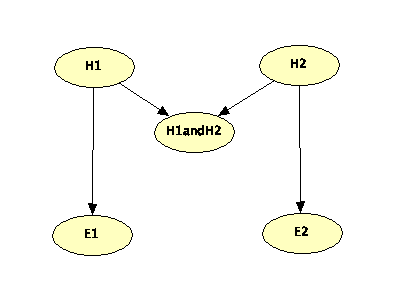
\includegraphics{conjunction-net.png}
\caption{Bayesian network for two pieces of evidence and a combined hypothesis.}
\label{network-conjunction}
\end{figure}

\hypertarget{specific-narratives-ideas-of-a-solution-to-theoretical-difficulties}{%
\section{Specific Narratives {[}IDEAS OF A SOLUTION TO THEORETICAL
DIFFICULTIES{]}}\label{specific-narratives-ideas-of-a-solution-to-theoretical-difficulties}}

MARCELLO: I AM NOW HAVING SECOND THOUGHTS (AGAIN!) ABOUT THE STRUCTURE
OF THIS CHAPTER. I FEEL THAT IN THIS CHAPTER WE SHOULD ONLY DESCRIBE THE
BASIC IDEA FOR A PROBABILISTIC SOLUTION TO NAKED STATS AND CONJUCTION. I
THINK I HAVE A SENSE OF WHAT THIS SOLUTION SHOULD LOOK LIKE. THERE WILL
THEN BE ANOTHER CHAPTER IN WHICH THIS ROUGH, INFORMAL IEDAS IS SPELLED
OUT FORMALLY USING BAYESIAN NETWORKS, BUT THAT CAN WAIT LATER WHEN WE
WRITE THE BOOK.

SO, THEN, THERE WOUDL BE ANOTHER CHAPTER IN WHICH WE DISCUSS AND REJECT
THE LIKELIHOOD RATIO APPROACH.

SO, BASICALLY, NOW WE HAVE TEH FOLLOWING SAMPLE CHAPTERS:

\begin{enumerate}
\def\labelenumi{\arabic{enumi}.}
\item
  DISCUSSIONS OF THRESHOLDS AS ANALYTICAL TOOLS, UTILITY, ERROR, ETC.
  (USE LOT OF STUFF FROM ORGINAL SEP ENTRY)
\item
  THEORETICAL DIFFICULTIES WITH THRESHOLD AND THE PROBABILISTIC
  SOLUTIONS (I.E. NARRATIVES)
\item
  REJECTION OF LIKELIHOOD RATIOS AS A GOOD SOLUTION TO THE THEORETICAL
  DIFFICULTIES
\end{enumerate}

So far we have assumed the most natural probabilistic interpretation of
proof standards, one that posits a threshold on the posterior
probabilities of a generic hypothesis such as guilt or civil liability.
In criminal cases, the requirement is formulated as follows: guilt is
proven beyond a reasonable doubt provided \(\Pr(G | E)\) is above a
suitable threshold, say 95\%. The threshold IS lower in civil trials.
Civil liability is proven by preponderance provided \(\Pr(L | E)\) is
above a suitable threshold, say 50\%. The claim that the defendant is
guilty or civilly liable can be replaced by a more fine-grained
hypothesis, call it \(H_p\), the hypothesis put foward by the prosecutor
(or the plaintiff in a civil case), for example, the hypothesis that the
defendant killed the victim with a firearm while bulglarizing the
victim's apartment. \(H_p\) can be any hypothesis which, if true, would
entail the defendanat is civilly or criminally liable (according to the
governing law). Hypothesis \(H_p\) is a more precise description of what
happened that establishes, if true, the defendant's guilt or civil
liability. In defining proof standards, instead of saying -- somewhat
generically -- that \(\pr{G | E}\) or \(\pr{L | E}\) should be above a
suitable threshold, a probabilistic interpretation could read: civil or
criminal liabbility is proven beyond a reasonable doubt provided
\(\Pr(H_d | E)\) is above a suitable threshold.

This variation may appear inconsequential. But we argue -- perhpas
surprisingly -- it can address the naked statistical evidence problem
and the difficulty about conjunction. Consider the prisoner
hypothetical. It is true that the naked statistics make him 99\% likely
to be guilty, that is, \(\pr{G | E_s}\). It is 99\% likely that he is
one the prisoners who attacked and killed the guard. Notice that this a
generic claim. It is odd for the prosecution to simply assert that the
prisoner was one of those who killed the guard, without saying what he
did, how he partook in the killing, what role he played in the attack,
etc. If the prosecution offerred a more specific incriminating
hypothesis, call it \(H_p\), the probability \(\pr{H_p | E_{s}}\) of
this hypothesis based on the naked statistical evidence \(E_s\) would be
well below 99\%, even though \(\pr{G | E_s}=99\%\). The fact the
prisoner on trial is most likely guilty is an artifact of the choice of
a generic hypothesis \(G\). When this hypthesis is made more specific --
as it should be -- this probability drops significantly. A more detailed
defense of this argument is provided in the rest of this chapter.

Consider now the difficulty about conjunction, focusing again on
criminal cases for the sake of concreteness. This difficulty assumes
that prosecutors should establish each element of a crime in isolation.
If they manage to prove each element to the desired standard, they have
meet their burden. This is an artificial view of legal proof. Consider a
Washington statute about negligent driving:

\begin{quote}
(1)(a) A person is guilty of negligent driving in the first degree if he or she operates a motor vehicle in a manner that is both negligent and endangers or is likely to endanger any person or property, and exhibits the effects of having consumed liquor or marijuana or any drug or exhibits the effects of having inhaled or ingested any chemical, whether or not a legal substance, for its intoxicating or hallucinatory effects. RCW 46.61.5249
\end{quote}

\noindent In other words, a prosecutor who wishes to establish beyond a
reasonable doubt that the defendant is guilty of negligent driving
should establish:

\begin{quote}
(a) the the defendant operated a vehicle
(b) that, in operating a vehicle, the defendant did so in  negligente manner
(c) that, in operating a vechicle, the defendant did so in a manner likely to endanger a person pr property
(d) that the defendant -- presumably, immediately after the incident -- exihibited the signs of intoxication by liquor or drugs
\end{quote}

\noindent These four claims form a common narratives about what
happenned. NEED TO COMPLETe THIS. BASIC IDEA IS THAT, FIRST, YOU
ESTABLISH THE NARTRATIVES, AND, SECOND, THE NARRATIVE IF TRUE PROVES
EACH ELEMENT. SO TO PROVE EACH ELEMENT SIMPLY MEANS TO PROVE A
NARRARTIVE FROM WHICH ALL ELEMENTS FOLLOW DEDUCTIVELY. THERE IS NO PINT
IN THIKING ABOUT WHETHER EACH ELEMENT HAS BEEN PROVEN.

\hypertarget{the-comparative-stratgey}{%
\section{The comparative stratgey}\label{the-comparative-stratgey}}

Instead of thinking in terms of absolute probability threshold, standard
of proof can be understood comparatively (Cheng, 2012). Say the
prosecutor or the plaintiff puts foward a hypthesis \(H_p\) about what
happened. The defense offers an alternative hypothesis about what
happened, call \(H_d\). This may be more common in civil than criminal
trials. On this approach, rather than directly evaluating the
probability of \(H_\Pi\) given the evidence and comparing it to a
threshold, we compare the support that the evidence provides for these
hypotheses, and decide for the one for which the evidence provides
better support. More specifically,given a body of evidence \(E\) and two
competing hypotheses \(H_p\) and \(H_d\), the probability
\(\pr{H_p | E}\) should be suitably higher than \(\pr{H_d | E}\), or in
other words, the ratio \(\frac{\Pr(H_p | E)}{\Pr(H_d | E)}\) should be
above a suitable threshold. Presumably, the ratio threshold shoud be
higher for criminal than civil cases. In fact, in civil cases it seems
enough to require that the ratio \(\frac{\Pr(H_p | E)}{\Pr(H_d | E)}\)
be avove 1, or in other words, \(\pr{H_p | E}\) should be higher than
\(\pr{H_d | E}\). Note that \(H_p\) and \(H_d\) need not be one the
negation of the other If they are one the negation of the other, then
\(\frac{\pr{H_p | E}}{\pr{H_d | E}}>1\) implies that
\(\pr{H_p | E}>50\%\), the standard probabilistic intepretation of the
preponderemca standard.

Cheng motivates this approach by the following considerations. Suppose
that if the decision is correct, no costs result, but incorrect
decisions have their price. Let us say that if the defendant is right
and we find against them, the cost is \(c_1\), and if the plaintiff is
right and we find against them, the cost is \(c_2\):

\begin{center}
\begin{tabular}
{@{}llll@{}}
\toprule
& & \multicolumn{2}{c}{Decision}\\
& &  $D_\Delta$ & $D_\Pi$ \\
\cmidrule{3-4}
\multirow{2}{*}{Truth} &  $H_\Delta$    & $0$    & $c_1$\\
                       &  $H_\Pi$       &  $c_2$   & $0$ \\ 
\bottomrule
\end{tabular}
\end{center}

Intuitively, it seems that we want a decision rule which minimizes the
expected cost. Say that given our total evidence \(E\) the relevant
conditional probabilities are:

\vspace{-6mm}

\begin{align*}
p_\Delta &= \pr{H_\Delta \vert E} \\
p_\Pi & = \pr{H_\Pi \vert E}
\end{align*} \noindent The expected costs for deciding that \(H_\Delta\)
and \(H_\Pi\), respectively, are: \begin{align*}
E(D_\Delta) & = p_\Delta 0 + p_\Pi c_2 = c_2p_\Pi\\
E(D_\Pi) & = p_\Delta c_1 + p_\Pi 0 = c_1 p_\Delta
\end{align*} \noindent For this reason, on these assumptions, we would
like to choose \(H_\Pi\) just in case \(E(D_\Pi) < E(D_\Delta)\). This
condition is equivalent to:

\vspace{-6mm}

\begin{align}
\nonumber c_1p_\Delta &< c_2p_\Pi \\
\nonumber c_1 & < \frac{c_2p_\Pi}{p_\Delta}\\
\label{eq:cheng_frac1}\frac{c_1}{c_2} & < \frac{p_\Pi}{p_\Delta}
\end{align}

\noindent Cheng (2012) (1261) insists:

\begin{quote}
At the same time, in a civil trial, the legal system expresses no preference between finding erroneously for the plaintiff (false positives) and finding erroneously for the defendant (false negatives). The costs $c_1$ and $c_2$ are thus equal\dots
\end{quote}

\noindent If we grant this assumption, \(c_1=c_2\),
\eqref{eq:cheng_frac1} reduces to:

\vspace{-6mm}

\begin{align}
\nonumber 1 &< \frac{p_\Pi}{p_\Delta} \\
\label{eq:cheng_comp1} p_\Pi &> p_\Delta 
\end{align} \noindent That is, in standard civil litigation we are to
find for the plaintiff just in case \(H_\Pi\) is more probable given the
evidence than \(H_\Delta\), which seems plausible.

This instruction is somewhat more general than the usual suggestion of
the preponderance standard in civil litigation, according to which the
court should find for the plaintiff just in case
\(\pr{H_\Pi\vert E} >0.5\). This threshold, however, results from
\eqref{eq:cheng_comp1} if it so happens that \(H_\Delta\) is
\(\n H_\Pi\), that is, if the defendant's claim is simply the negation
of the plaintiff's thesis. By no means, Cheng argues, this is always the
case.

How is RLP supposed to handle DAC? Consider an imaginary case, used by
Cheng to discuss this issue. In it, the plaintiff claims that the
defendant was speeding (\(S\)) and that the crash caused her neck injury
(\(C\)). Thus, \(H_\Pi\) is \(S\et C\). Suppose that given total
evidence \(E\), the conjuncts, taken separately, meet the decision
standard of RLP: \begin{align}
 \nonumber 
 \frac{\pr{S\vert E}}{\pr{\n S \vert E}} > 1   & & \frac{\pr{C\vert E}}{\pr{\n C \vert E}} > 1
\end{align} \noindent The question, clearly, is whether
\(\frac{\mathtt{P}(S\et C\vert E)}{H_\Delta \vert E}>1\). But to answer
it, we have to decide what \(H_\Delta\) is. This is the point where
Cheng's remark that \(H_\Delta\) isn't normally simply \(\n H_\Pi\).
Instead, he insists, there are three alternative defense scenarios:
\(H_{\Delta_1}= S\et \n C\), \(H_{\Delta_2}=\n S \et C\), and
\(H_{\Delta_3}=\n S \et \n C\). How does \(H_\Pi\) compare to each of
them? Cheng (assuming independence) argues:
\begin{align}\label{eq:cheng-multiplication}
\frac{\pr{S\et C\vert E}}{\pr{S\et \n C\vert E}} & = \frac{\pr{S\vert E}\pr{C\vert E}}{\pr{S \vert E}\pr{\n C \vert E}}  =\frac{\pr{C\vert E}}{\pr{\n C \vert E}} > 1 \\
\nonumber
\frac{\pr{S\et C\vert E}}{\pr{\n S\et C\vert E}} & = \frac{\pr{S\vert E}\pr{C\vert E}}{\pr{\n S \vert E}\pr{C\vert E}}  = \frac{\pr{S\vert E}}{\pr{\n S \vert E}} > 1 \\
\nonumber
\frac{\pr{S\et C\vert E}}{\pr{\n S\et \n C\vert E}} & = \frac{\pr{S\vert E}\pr{C\vert E}}{\pr{\n S \vert E}\pr{\n C \vert E}}   > 1 
\end{align}

\noindent It seems that whatever the defense story is, it is less
plausible than the plaintiff's claim. So, at least in this case,
whenever elements of a plaintiff's claim satisfy the decision standard
proposed by RLP, then so does their conjunction.

Similarly, RLP is claimed to handle the gatecrasher paradox. It is
useful to think about the problem in terms of odds and likelikoods,
where the \emph{prior odds} (before evidence \(E\)) of \(H_\Pi\) as
compared to \(H_\Delta\), are \(\frac{\pr{H_\Pi}}{\pr{H_\Delta}}\), the
posterior odds of \(H_\Delta\) given \(E\) are
\(\frac{\pr{H_\Pi \vert E}}{\pr{H_\Delta \vert E}}\), and the
corresponding likelihood ratio is
\(\frac{\pr{E\vert H_\Pi}}{\pr{E\vert H_\Delta}}\).

Now, with this notation the \emph{odds form of Bayes' Theorem} tells us
that the posterior odds equal the likelihood ratio multiplied by prior
odds: \begin{align*}
\frac{\pr{H_\Pi \vert E}}{\pr{H_\Delta \vert E}} & = 
\frac{\pr{E\vert H_\Pi}}{\pr{E\vert H_\Delta}} 
\times \frac{\pr{H_\Pi}}{\pr{H_\Delta}}
 \end{align*} \noindent [@cheng2012reconceptualizing: 1267] insists that
in civil trials the prior probabilities should be equal. Granted this
assumption, prior odds are 1, and we have:
\begin{align}\label{eq:cheng_simple_odds}
\frac{\pr{H_\Pi \vert E}}{\pr{H_\Delta \vert E}} & = 
\frac{\pr{E\vert H_\Pi}}{\pr{E\vert H_\Delta}} 
 \end{align} This means that our original task of establishing that the
left-hand side is greater than 1 now reduces to establishing that so is
the right-hand side, which means that RLP tells us to convict just in
case: \begin{align}\label{eq:Cheng:compar2}
\pr{E\vert H_\Pi} &> \pr{E\vert H_\Delta}
\end{align} Thus, \eqref{eq:Cheng:compar2} tells us to convict just in
case \(LR(E)>1\).

Now, in the case of the gatecrasher paradox, our evidence is
statistical. In our variant
\(E\)=\texttt{991\ out\ of\ 1000\ spectators\ gatecrashed\textquotesingle{}\textquotesingle{}.\ Now\ pick\ a\ random\ spectator,\ call\ him\ Tom,\ and\ let\ \$H\_\textbackslash{}Pi\$=}Tom
gatecrashed.'' (Cheng, 2012: 1270) insists:

\begin{quote}
But whether the audience member is a lawful patron or a gatecrasher does not change the probability of observing the evidence presented.
\end{quote}

\noindent So, on his view, in such a case,
\(\pr{E\vert H_\Pi}=\pr{E\vert H_\Delta}\), the posterior odds are, by
\eqref{eq:cheng_simple_odds}, equal to 1, and conviction is unjustified.

There are various issues with how RLP has been deployed to resolve the
difficulties that CLP and TLP run into.\\
First of all, to move from \eqref{eq:cheng_frac1} to
\eqref{eq:cheng_comp1}, Cheng assumes that the costs of wrongful
decision is the same, be it conviction or acquittal. This is by no means
obvious. If a poor elderly lady sues a large company for serious health
damage that it supposedly caused, leaving her penniless if the company
is liable is definitely not on a par with mistakenly making the company
lose a small percent of their funds. Even in cases where such costs are
equal, careful consideration and separate argument is needed. If, for
instance, \(c_1=5c_2\), we are to convict just in case
\(5<\frac{p_\Pi}{p_\Delta}\). This limits the applicability of Cheng's
reasoning about DAC, because his reasoning, if correct (and I will argue
that it is not correct later on), yields only the result that the
relevant posterior odds are greater than 1, not that they are greater
than 5. The difficulty, however, will not have much impact on Cheng's
solution of the gatecrasher paradox, as long as \(c_1\leq c_2\). This is
because his reasoning, if correct (and I will argue that it is not
correct later on), establishes that the relevant posterior odds are
below 1, and so below any higher threshold as well.

Secondly, Cheng's resolution of DAC uses another suspicious assumption.
For \eqref{eq:cheng-multiplication} to be acceptable we need to assume
that the following pairs of events are independent conditionally on
\(E\): \(\la S, C\ra\), \(\la S, \n C\ra\), \(\la \n S, C\ra\),
\(\la \n S, \n C\ra\). Otherwise, Cheng would not be able to replace
conditional probabilities of corresponding conjunctions with the result
of multiplication of conditional probabilities of the conjuncts. But it
is far from obvious that speeding and neck injury are independent. If,
for instance, the evidence makes it certain that if the car was not
speeding, the neck injury was not caused by the accident,
\(\pr{\n S\et C\vert E}=0\), despite the fact that
\(\pr{\n S \vert E}\pr{C\vert E}\) does not have to be \(0\)!

Without independence, the best that we can get, say for the first line
of \eqref{eq:cheng-multiplication}, is: \begin{align*}
\pr{S\et C\vert E} & = \pr{C\vert E}\pr{S\vert C \et E}\\
\pr{S\et \n C\vert E} & = \pr{\n C\vert E}\pr{S\vert  \n C \et E}
\end{align*} and even if we know that
\(\pr{C\vert E}>\pr{\n C\vert E}\), this tells us nothing about the
comparison of \(\pr{S\et C\vert E}\) and \(\pr{S\et \n C\vert E}\),
because the remaining factors can make up for the former inequality.

Perhaps even more importantly, much of the heavy lifting here is done by
the strategic splitting of the defense line into multiple scenarios. The
result is rather paradoxical. For suppose \(\pr{H_\Pi\vert E}=0.37\) and
the probability of each of the defense lines given \(E\) is \(0.21\).
This means that \(H_\Pi\) wins with each of the scenarios, so, according
to RLP, we should find for the plaintiff. On the other hand, how eager
are we to convict once we notice that given the evidence, the accusation
is rather false, because \(\pr{\n H_\Pi\vert E}=0.63\)?

The problem generalizes. If, as here, we individualize scenarios by
boolean combinations of elements of a case, the more elements there are,
into more scenarios \(\n H_\Pi\) needs to be divided. This normally
would lead to the probability of each of them being even lower (because
now \(\pr{\n H_\Pi}\) needs to be ``split'' between more different
scenarios). So, if we take this approach seriously, the more elements a
case has, the more at disadvantage the defense is. This is clearly
undesirable.

\hypertarget{the-likelihood-strategy}{%
\section{The likelihood strategy}\label{the-likelihood-strategy}}

Focusing on posterior probabilities is not the only approach that legal
probabilists can pursue. By Bayes' theorem, the following holds, using
\(G\) and \(I\) as competing hypotheses:

\[ \frac{\Pr(G | E)}{\Pr(I | E)} = \frac{\Pr(E | G)}{\Pr(E | I)} \times \frac{\Pr(G)}{\Pr(I)},\]

or using \(H_p\) and \(H_d\) as competing hypotheses,

\[ \frac{\Pr(H_p | E)}{\Pr(H_d | E)} = \frac{\Pr(E | H_p)}{\Pr(E | H_d)} \times \frac{\Pr(H_p)}{\Pr(H_d)},\]

or in words

\[ \textit{posterior odds} = \textit{likelihood ratio} \times \textit{prior odds}.\]

A difficult problem is to assign numbers to the prior probabiliteis such
as \(\Pr(G)\) or \(\Pr(H_p)\), or priors odds such as
\(\frac{\Pr(G)}{\Pr(I)}\) or \(\frac{\Pr(H_p)}{\Pr(H_d)}\).

DISCUSS DIFFICULTIES ABOUT ASSIGNING PRIORS! WHERE? CAN WE USE IMPRECISE
PROBABILKITIES T TALK ABOUT PRIORS -- I.E. LOW PRIORS = TOTAL IGNORANCE
= VERY IMPRECISE (LARGE INTERVAL) PRIORS? THE PROBLME WITH THIS WOULD BE
THAT THERE IS NO UPDSATING POSSIBLE. ALL UPDATING WOULD STILL GET BACK
TO THE STARTING POINT. DO YOU HAVE AN ANSWER TO THAT? WOULD BE
INTERETSING TO DISCUSS THIS!

Given these difficulties, both practical and theoretical, one option is
to dispense with priors altogether. This is not implausible. Legal
disputes in both criminal and civil trials should be decided on the
basis of the evidence presented by the litigants. But it is the
likelihood ratio -- not the prior ratio -- that offers the best measure
of the overall strength of the evidece presented. So it is all too
natural to focus on likekihood ratios and leave the priors out of the
picture. If this is the right, the question is, how would a
probabilistic interpretation of standards of proof based on the
likelihood rato look like? At its simplest, this stratgey will look as
follows. Recall our discussion of expected utility theory:

\[ \text{convict provided}           \frac{cost(CI)}{cost(AG)} < \frac{\Pr(H_p | E)}{\Pr(H_d | E )}, \]

which is equivalent to

\[ \text{convict provided}           \frac{cost(CI)}{cost(AG)} < \frac{\Pr(E | H_p)}{\Pr(E | H_d)} \times \frac{\Pr(H_p)}{\Pr(H_d)}.\]

By rearraing the terms,

\[ \text{convict provided}  \frac{\Pr(E | H_p)}{\Pr(E | H_d)} > \frac{\Pr(H_d)}{\Pr(H_p)} \times     \frac{cost(CI)}{cost(AG)} .\]

Then, on this intepretation, the likelihood ratio should be above a
suitable threshold that is a function of the cost ratio and the prior
ratio. The outstanding question is how this threshold is to be
determined.

\hypertarget{kaplow}{%
\subsection{Kaplow}\label{kaplow}}

Quite independently, a similar approach to juridical decisions has been
proposed by Kaplow (2014) -- we'll call it
\textbf{decision-theoretic legal probabilism (DTLP)}. It turns out that
Cheng's suggestion is a particular case of this more general approach.
Let \(LR(E)=\pr{E\vert H_\Pi}/\pr{E\vert H_\Delta}\). In whole
generality, DTLP invites us to convict just in case \(LR(E)>LR^\star\),
where \(LR^\star\) is some critical value of the likelihood ratio.

Say we want to formulate the usual preponderance rule: convict iff
\(\pr{H_\Pi\vert E}>0.5\), that is, iff
\(\frac{\pr{H_\Pi\vert E}}{\pr{H_\Delta\vert E}}>1\). By Bayes' Theorem
we have:

\vspace{-6mm}

\begin{align*}
\frac{\pr{H_\Pi\vert E}}{\pr{H_\Delta\vert E}} =  \frac{\pr{H_\Pi}}{\pr{H_\Delta}}\times \frac{\pr{E\vert H_\Pi}}{\pr{E\vert H_\Delta}} &>1 \Leftrightarrow\\
  \Leftrightarrow \frac{\pr{E\vert H_\Pi}}{\pr{E\vert H_\Delta}} &> \frac{\pr{H_\Delta}}{\pr{H_\Pi}} 
 \end{align*} \noindent So, as expected, \(LR^\star\) is not unique and
depends on priors. Analogous reformulations are available for thresholds
other than \(0.5\).

Kaplow's point is not that we can reformulate threshold decision rules
in terms of priors-sensitive likelihood ratio thresholds. Rather, he
insists, when we make a decision, we should factor in its consequences.
Let \(G\) represent potential gain from correct conviction, and \(L\)
stand for the potential loss resulting from mistaken conviction. Taking
them into account, Kaplow suggests, we should convict if and only if:

\vspace{-6mm}

\begin{align}
\label{eq:Kaplow_decision}
\pr{H_\Pi\vert E}\times G > \pr{H_\Delta\vert E}\times L
\end{align} \noindent Now, \eqref{eq:Kaplow_decision} is equivalent to:

\vspace{-6mm}

\begin{align}
\nonumber
\frac{\pr{H_\Pi \vert E}}{\pr{H_\Delta \vert E}} & > \frac{L}{G}\\
\nonumber
\frac{\pr{H_\Pi}}{\pr{H_\Delta}} \times \frac{\pr{E\vert H_\Pi}}{\pr{E\vert H_\Delta}} &> \frac{L}{G}\\
\nonumber
\frac{\pr{E\vert H_\Pi}}{\pr{E\vert H_\Delta}}  & > \frac{\pr{H_\Delta}}{\pr{H_\Pi}} \times \frac{L}{G}\\
\label{eq:Kaplow_decision2} LR(E)  & > \frac{\pr{H_\Delta}}{\pr{H_\Pi}} \times \frac{L}{G}
\end{align}

\noindent This is the general format of Kaplow's decision standard.

\hypertarget{dawid}{%
\subsection{Dawid}\label{dawid}}

Here is a slightly different perspective, due to Dawid (1987), that also
suggests that juridical decisions should be likelihood-based. The focus
is on witnesses for the sake of simplicity. Imagine the plaintiff
produces two independent witnesses: \(W_A\) attesting to \(A\), and
\(W_B\) attesting to \(B\). Say the witnesses are regarded as \(70\%\)
reliable and \(A\) and \(B\) are probabilistically independent, so we
infer \(\pr{A}=\pr{B}=0.7\) and \(\pr{A\et B}=0.7^2=0.49\).

But, Dawid argues, this is misleading, because to reach this result we
misrepresented the reliability of the witnesses: \(70\%\) reliability of
a witness, he continues, does not mean that if the witness testifies
that \(A\), we should believe that \(\pr{A}=0.7\). To see his point,
consider two potential testimonies:

\begin{center}
\begin{tabular}
{@{}ll@{}}
\toprule
  $A_1$ & The sun rose today. \\
   $A_2$ & The sun moved backwards through the sky today.\\
\bottomrule
\end{tabular}
\end{center}

\noindent     Intuitively, after hearing them, we would still take
\(\pr{A_1}\) to be close to 1 and \(\pr{A_2}\) to be close to 0, because
we already have fairly strong convictions about the issues at hand. In
general, how we should revise our beliefs in light of a testimony
depends not only on the reliability of the witness, but also on our
prior
convictions.\footnote{An issue that Dawid does not bring up is the interplay between our priors and our assessment of the reliability of the witnesses. Clearly, our posterior assessment of the credibility of the witness who testified $A_2$ will be lower than that of the other witness.}
And this is as it should be: as indicated by Bayes' Theorem, one and the
same testimony with different priors might lead to different posterior
probabilities.

So far so good. But how should we represent evidence (or testimony)
strength then? Well, one pretty standard way to go is to focus on how
much it contributes to the change in our beliefs in a way independent of
any particular choice of prior beliefs. Let \(a\) be the event that the
witness testified that \(A\). It is useful to think about the problem in
terms of \emph{odds, conditional odds (O)} and
\emph{likelihood ratios (LR)}:
\begin{align*} O(A)  & = \frac{\pr{A}}{\pr{\n A}}\\
 O(A\vert a) &= \frac{\pr{A\vert a}}{\pr{\n A \vert a}}  \\
 LR(a\vert A) &= \frac{\pr{a\vert A}}{\pr{a\vert \n A}}. 
\end{align*}

Suppose our prior beliefs and background knowledge, before hearing a
testimony, are captured by the prior probability measure
\(\prr{\cdot}\), and the only thing that we learn is \(a\). We're
interested in what our \emph{posterior} probability measure,
\(\prp{\cdot}\), and posterior odds should then be. If we're to proceed
with Bayesian updating, we should have:

\vspace{-6mm}

\begin{align*}
 \frac{\prp{A}}{\prp{\n A}} & = \frac{\prr{A\vert a}}{\prr{\n A\vert a}}
 =
 \frac{\prr{a\vert A}}{\prr{a\vert \n A}}
 \times
 \frac{\prr{A}}{\prr{\n A}}
  \end{align*} that is,

\vspace{-6mm}

\begin{align}
 \label{bayesodss2}
 O_{posterior}(A)& = O_{prior}(A\vert a) = \!\!\!\!\!  \!\!\!\!\!  \!\! \!\!  \underbrace{LR_{prior}(a\vert A)}_{\mbox{\footnotesize conditional likelihood ratio}}  \!\!\!\!\!   \!\!\!\!\!  \!\! \!\!   \times  O_{prior}(A)
 \end{align}

The conditional likelihood ratio seems to be a much more direct measure
of the value of \(a\), independent of our priors regarding \(A\) itself.
In general, the posterior probability of an event will equal to the
witness's reliability in the sense introduced above only if the prior is
\(1/2\).\footnote{Dawid gives no general argument, but it is not too hard to  give one. Let $rel(a)=\pr{a\vert A}=\pr{\n a\vert \n A}$. We have in the background $\pr{a\vert \n A}=1-\pr{\n a\vert \n A}=1-rel(a)$.
 We want to find the condition under which $\pr{A\vert a} = \pr{a\vert A}$. Set $\pr{A}=p$ and  start with Bayes' Theorem and the law of total probability, and go from there:
 \begin{align*}
 \pr{A\vert a}& = \pr{a\vert A}\\
 \frac{\pr{a\vert A}p}{\pr{a\vert A}p+\pr{a\vert \n A}(1-p)} &= \pr{a\vert A} \\
 \pr{a\vert A}p & = \pr{a\vert A}[\pr{a\vert A}p+\pr{a\vert \n A}(1-p)]\\
 p & = \pr{a\vert A}p + \pr{a\vert \n A} - \pr{a\vert \n A}p\\
 p &= rel(a) p + 1-rel(a)- (1-rel(a))p\\
 p & = rel(a)p +1 - rel(a) -p +rel(a)p \\
 2p & =  2rel(a)p + 1 - rel(a)  \\
 2p - 2 rel(a)p & = 1-rel(a)\\
 2p(1-rel(a)) &= 1-rel(a)\\
 2p & = 1
 \end{align*}

\noindent  First we multiplied both sides by the denominator. Then we divided both sides by $\pr{a\vert A}$ and multiplied on the right side. Then we used our background notation and information. Next, we manipulated the right-hand side algebraically and  moved  $-p$ to the left-hand side. Move $2rel(a)p$ to the left and manipulate the result algebraically to get to the last line.}

\hypertarget{likelihood-and-dac}{%
\subsection{Likelihood and DAC}\label{likelihood-and-dac}}

But how does our preference for the likelihood ratio as a measure of
evidence strength relate to DAC? Let's go through Dawid's reasoning.

A sensible way to probabilistically interpret the \(70\%\) reliability
of a witness who testifies that \(A\) is to take it to consist in the
fact that the probability of a positive testimony if \(A\) is the case,
just as the probability of a negative testimony (that is, testimony that
\(A\) is false) if \(A\) isn't the case, is
0.7:\footnote{In general setting, these are called the \emph{sensitivity} and \emph{specificity} of a test (respectively), and they don't have to be equal. For instance, a degenerate test for an illness which always responds positively, diagnoses everyone as ill, and so has sensitivity 1, but specificity 0.}
\[\prr{a\vert A}=\prr{\n a\vert\n  A}=0.7.\]
\noindent   \(\prr{a\vert \n A}=1- \prr{\n a\vert \n A}=0.3\), and so
the same information is encoded in the appropriate likelihood ratio:
\[LR_{prior}(a\vert A )=\frac{\prr{a\vert A}}{\prr{a\vert \n A}}= \frac{0.7}{0.3}\]

Let's say that \(a\) \emph{provides (positive) support} for \(A\) in
case \[O_{posterior}(A)=O_{prior}(A\vert a)> O_{prior}(A)\]
\noindent  that is, a testimony \(a\) supports \(A\) just in case the
posterior odds of \(A\) given \(a\) are greater than the prior odds of
\(A\) (this happens just in case \(\prp{A}>\prr{A}\)). By
\eqref{bayesodss2}, this will be the case if and only if
\(LR_{prior}(a\vert A)>1\).

One question that Dawid addresses is this: assuming reliability of
witnesses \(0.7\), and assuming that \(a\) and \(b\), taken separately,
provide positive support for their respective claims, does it follow
that \(a \et b\) provides positive support for \(A\et B\)?

Assuming the independence of the witnesses, this will hold in
non-degenerate cases that do not involve extreme probabilities, on the
assumption of independence of \(a\) and \(b\) conditional on all
combinations: \(A\et B\), \(A\et \n B\), \(\n A \et B\) and
\(\n A \et \n B\).\footnote{Dawid only talks about the independence of witnesses without reference to  conditional independence. Conditional independence does not follow from independence, and it is the former that is needed here (also, four non-equivalent different versions of it).}\(^,\)\textasciitilde{}\footnote{In terms of notation and derivation in the optional content that will follow, the claim holds  if and only if $28 > 28 p_{11}-12p_{00}$.  This inequality is not  true for all admissible values of $p_{11}$ and $p_{00}$. If $p_{11}=1$ and $p_{00}=0$, the sides are equal. However, this is a rather degenerate example. Normally, we are  interested in cases where $p_{11}< 1$. And indeed, on this assumption, the inequality holds.}

Let us see why the above claim holds. The calculations are my
reconstruction and are not due to Dawid. The reader might be annoyed
with me working out the mundane details of Dawid's claims, but it turns
out that in the case of Dawid's strategy, the devil is in the details.
The independence of witnesses gives us: \begin{align*}
 \pr{a \et b \vert A\et B}& =0.7^2=0.49\\
 \pr{a \et b \vert A\et \n B}& =  0.7\times 0.3=0.21\\
 \pr{a \et b \vert \n A\et B}& =  0.3\times 0.7=0.21\\
 \pr{a \et b \vert \n A\et \n B}& =  0.3\times 0.3=0.09
 \end{align*} Without assuming \(A\) and \(B\) to be independent, let
the probabilities of \(A\et B\), \(\n A\et B\), \(A\et \n B\),
\(\n A\et \n B\) be \(p_{11}, p_{01}, p_{10}, p_{00}\). First, let's see
what \(\pr{a\et b}\) boils down to.

By the law of total probability we have:
\begin{align}\label{eq:total_lower}
 \pr{a\et b} & = 
                     \pr{a\et b \vert A \et B}\pr{A\et B} + \\ &  \nonumber
                     +\pr{a\et b \vert A \et \n B}\pr{A\et \n B} \\ &  \nonumber
 + \pr{a\et b \vert \n A \et B}\pr{\n A\et B} + \\ & \nonumber
                     + \pr{a\et b \vert \n A \et \n B}\pr{\n A\et \n B}
 \end{align} \noindent which, when we substitute our values and
constants, results in: \begin{align*}
                     & = 0.49p_{11}+0.21(p_{10}+p_{01})+0.09p_{00}
 \end{align*} Now, note that because \(p_{ii}\)s add up to one, we have
\(p_{10}+p_{01}=1-p_{00}-p_{11}\). Let us continue. \begin{align*}
    & = 0.49p_{11}+0.21(1-p_{00}-p_{11})+0.09p_{00} \\
                     & = 0.21+0.28p_{11}-0.12p_{00}
 \end{align*}

Next, we ask what the posterior of \(A\et B\) given \(a\et b\) is (in
the last line, we also multiply the numerator and the denominator by
100). \begin{align*}
 \pr{A\et B\vert a \et b} & =
         \frac{\pr{a\et b \vert A \et B}\pr{A\et B}}
             {\pr{a\et b}}\\
         & =
                     \frac{49p_{11}}
                           {21+28p_{11}-12p_{00}} 
         \end{align*}

In this particular case, then, our question whether
\(\pr{A\et B\vert a\et b}>\pr{A\et B}\) boils down to asking whether
\[\frac{49p_{11}}{21+28p_{11}-12p_{00}}> p_{11}\] that is, whether
\(28 > 28 p_{11}-12p_{00}\) (just divide both sides by \(p_{11}\),
multiply by the denominator, and manipulate algebraically).

Dawid continues working with particular choices of values and provides
neither a general statement of the fact that the above considerations
instantiate nor a proof of it. In the middle of the paper he says:

\begin{quote}
 Even under prior dependence, the combined support is always positive, in the sense that the posterior probability of the case always exceeds its prior probability\dots When the problem is analysed carefully, the `paradox' evaporates [pp. 95-7]\end{quote}

\noindent where he still means the case with the particular values that
he has given, but he seems to suggest that the claim generalizes to a
large array of cases.

The paper does not contain a precise statement making the conditions
required explicit and, \emph{a fortriori}, does not contain a proof of
it. Given the example above and Dawid's informal reading, let us develop
a more precise statement of the claim and a proof thereof.

\begin{fact}\label{ther:increase}
Suppose that  $rel(a),rel(b)>0.5$ and witnesses are independent conditional on all Boolean combinations of $A$ and $B$  (in a sense to be specified), and that none of the Boolean combinations of $A$ and $B$ has an extreme probability (of 0 or 1). It follows that  $\pr{A\et B \vert a\et b}>\pr{A\et B}$. (Independence of $A$ and $B$ is not required.)
\end{fact}

Roughly, the theorem says that if independent and reliable witnesses
provide positive support of their separate claims, their joint testimony
provides positive support of the conjunction of their claims.

Let us see why the claim holds. First, we introduce an abbreviation for
witness reliability:
\begin{align*}\mathbf{a} &=rel(a)=\pr{a\vert A}=\pr{\n a\vert \n A}>0.5\\ 
\mathbf{b} &=rel(b)=\pr{b\vert B}=\pr{\n b\vert \n A}>0.5
\end{align*} Our independence assumption means: \begin{align*}
\pr{a\et b \vert A\et B}  &= \mathbf{ab}\\
\pr{a\et b \vert A\et \n B} & = \mathbf{a(1-b)}\\
\pr{a\et b \vert \n A\et B}  & = \mathbf{(1-a)b}\\
\pr{a\et b \vert \n A\et \n  B}  & = \mathbf{(1-a)(1-b)}
\end{align*}

\vspace{-2mm}

Abbreviate the probabilities the way we already did:

\begin{center}
\begin{tabular}{ll}
$\pr{A\et B} = p_{11}$ & $\pr{A\et \n B} = p_{10}$\\
$\pr{\n A \et B} = p_{01}$ & $\pr{\n A \et \n B}=p_{00}$
\end{tabular}
\end{center}

Our assumptions entail \(0\neq p_{ij}\neq 1\) for \(i,j\in \{0,1\}\)
and: \begin{align}\label{eq:sumupto1}
p_{11}+p_{10}+p_{01}+p_{00}&=1
\end{align}

\noindent So, we can use this with \eqref{eq:total_lower} to get:
\begin{align}\label{eq:aetb}
\pr{a\et b} & =  \mathbf{ab}p_{11} + \mathbf{a(1-b)}p_{10}+\mathbf{(1-a)b}p_{01} + \mathbf{(1-a)(1-b)}p_{00}\\ \nonumber
& = p_{11}\mathbf{ab} + p_{10}(\mathbf{a}-\mathbf{ab}) + p_{01}(\mathbf{b}-\mathbf{ab})+p_{00}(1-\mathbf{b}-\mathbf{a}+\mathbf{ab})
\end{align}

Let's now work out what the posterior of \(A\et B\) will be, starting
with an application of the Bayes' Theorem: \begin{align} \nonumber
\pr{A\et B \vert a\et b} & = \frac{\pr{a\et b \vert A \et B}\pr{A\et B}}{\pr{a\et b}}
\\ \label{eq:boiled}
& = \frac{\mathbf{ab}p_{11}}{p_{11}\mathbf{ab} + p_{10}(\mathbf{a}-\mathbf{ab}) + p_{01}(\mathbf{b}-\mathbf{ab})+p_{00}(1-\mathbf{b}-\mathbf{a}+\mathbf{ab})}
\end{align} To answer our question we therefore have to compare the
content of \eqref{eq:boiled} to \(p_{11}\) and our claim holds just in
case: \begin{align*}
\frac{\mathbf{ab}p_{11}}{p_{11}\mathbf{ab} + p_{10}(\mathbf{a}-\mathbf{ab}) + p_{01}(\mathbf{b}-\mathbf{ab})+p_{00}(1-\mathbf{b}-\mathbf{a}+\mathbf{ab})} &> p_{11}
\end{align*} \begin{align*}
 \frac{\mathbf{ab}}{p_{11}\mathbf{ab} + p_{10}(\mathbf{a}-\mathbf{ab}) + p_{01}(\mathbf{b}-\mathbf{ab})+p_{00}(1-\mathbf{b}-\mathbf{a}+\mathbf{ab})} & > 1\end{align*}
\begin{align}  
 \label{eq:goal}
p_{11}\mathbf{ab} + p_{10}(\mathbf{a}-\mathbf{ab}) + p_{01}(\mathbf{b}-\mathbf{ab})+p_{00}(1-\mathbf{b}-\mathbf{a}+\mathbf{ab}) & < \mathbf{ab}
\end{align} Proving \eqref{eq:goal} is therefore our goal for now. This
is achieved by the following
reasoning:\footnote{Thanks to Pawel Pawlowski for working on this proof with me.}

\hspace{-7mm}
\resizebox{13.5cm}{!}{
\begin{tabular}{llr}
 1. & $\mathbf{b}>0.5,\,\,\, \mathbf{a}>0.5$ & \mbox{assumption}\\
 2. & $2\mathbf{b}>1,\,\,\, 2\mathbf{a}> 1$ & \mbox{from 1.}\\
 3. & $2\mathbf{ab}>\mathbf{a},\,\,\, 2\mathbf{ab}>\mathbf{b}$ & \mbox{multiplying by $\mathbf{a}$ and $\mathbf{b}$ respectively}\\
 4.  & $p_{10}2\mathbf{ab}>p_{10}\mathbf{a}$,\,\,\, $p_{01}2\mathbf{ab}>p_{01}\mathbf{b}$ & \mbox{multiplying by $p_{10}$ and $p_{01}$ respectively}\\
 5.  & $p_{10}2\mathbf{ab} +  p_{01}2\mathbf{ab} > p_{10}\mathbf{a} + p_{01}\mathbf{b}$ & \mbox{adding by sides, 3., 4.}\\
 6. & $1- \mathbf{b}- \mathbf{a} <0$ & \mbox{from 1.}\\
 7. & $p_{00}(1-\mathbf{b}-\mathbf{a})<0$ & \mbox{From 6., because $p_{00}>0$}\\
  8.  &  $p_{10}2\mathbf{ab} +  p_{01}2\mathbf{ab} > p_{10}\mathbf{a} + p_{01}\mathbf{b} + p_{00}(1-\mathbf{b}-\mathbf{a})$ & \mbox{from 5. and 7.}\\
  9.  & $p_{10}\mathbf{ab} + p_{10}\mathbf{ab} + p_{01}\mathbf{ab} + p_{01}\mathbf{ab} + p_{00}\mathbf{ab} - p_{00}\mathbf{ab}> p_{10}\mathbf{a} + p_{01}\mathbf{b} + p_{00}(1-\mathbf{b}-\mathbf{a})$ & \mbox{8., rewriting left-hand side}\\
  10.  & $p_{10}\mathbf{ab} + p_{01}\mathbf{ab}  + p_{00}\mathbf{ab} > - p_{10}\mathbf{ab}  -  p_{01}\mathbf{ab} + p_{00}\mathbf{ab} +  p_{10}\mathbf{a} + p_{01}\mathbf{b} + p_{00}(1-\mathbf{b}-\mathbf{a})$ &  \mbox{9., moving from left to right}\\
11. & $\mathbf{ab}(p_{10}+p_{01}+p_{00})> p_{10}(\mathbf{a}-\mathbf{ab})+p_{01}(\mathbf{b}-\mathbf{ab})+p_{00}(1-\mathbf{b}-\mathbf{a}+\mathbf{ab})$ & \mbox{10., algebraic manipulation}\\
12. & $\mathbf{ab}(1-p_{11})> p_{10}(\mathbf{a}-\mathbf{ab})+p_{01}(\mathbf{b}-\mathbf{ab})+p_{00}(1-\mathbf{b}-\mathbf{a}+\mathbf{ab})$ & \mbox{11. and equation \eqref{eq:sumupto1}}\\
13. & $\mathbf{ab}- \mathbf{ab}p_{11}> p_{10}(\mathbf{a}-\mathbf{ab})+p_{01}(\mathbf{b}-\mathbf{ab})+p_{00}(1-\mathbf{b}-\mathbf{a}+\mathbf{ab})$ & \mbox{12., algebraic manipulation}\\
14. & $\mathbf{ab}> \mathbf{ab}p_{11}+ p_{10}(\mathbf{a}-\mathbf{ab})+p_{01}(\mathbf{b}-\mathbf{ab})+p_{00}(1-\mathbf{b}-\mathbf{a}+\mathbf{ab})$ & \mbox{13., moving from left to right}\\
\end{tabular}}

\%\textbackslash{}end\{adjustbox\}

\vspace{1mm}

The last line is what we have been after.

\intermezzob

Now that we have as a theorem an explication of what Dawid informally
suggested, let's see whether it helps the probabilist handling of DAC.

\hypertarget{kaplow-1}{%
\subsection{Kaplow}\label{kaplow-1}}

On RLP, at least in certain cases, the decision rule leads us to
\eqref{eq:Cheng:compar2}, which tells us to decide the case based on
whether the likelihood ratio is greater than 1.

\footnote{Again, the name of the view is by no means standard, it is  just a term I coined to refer to various types of legal probabilism in a fairly uniform manner.}
While Kaplow did not discuss DAC or the gatecrasher paradox, it is only
fair to evaluate Kaplow's proposal from the perspective of these
difficulties.

Add here stuff from Marcello's Mind paper about the prisoner
hypothetical. Then, discuss Rafal's critique of the likelihood ratio
threshold and see where we end up.

\hypertarget{challenges-again}{%
\section{Challenges (again)}\label{challenges-again}}

\hypertarget{likelihood-ratio-and-the-problem-of-the-priors}{%
\subsection{Likelihood ratio and the problem of the
priors}\label{likelihood-ratio-and-the-problem-of-the-priors}}

\hypertarget{dawids-likelihood-strategy-doesnt-help}{%
\subsection{Dawid's likelihood strategy doesn't
help}\label{dawids-likelihood-strategy-doesnt-help}}

Recall that DAC was a problem posed for the decision standard proposed
by TLP, and the real question is how the information resulting from Fact
\ref{ther:increase} can help to avoid that problem. Dawid does not
mention any decision standard, and so addresses quite a different
question, and so it is not clear that `\texttt{the}paradox'
evaporates'', as Dawid suggests.

What Dawid correctly suggests (and we establish in general as Fact
\ref{ther:increase}) is that the support of the conjunction by two
witnesses will be positive as soon as their separate support for the
conjuncts is positive. That is, that the posterior of the conjunction
will be higher that its prior. But the critic of probabilism never
denied that the conjunction of testimonies might raise the probability
of the conjunction if the testimonies taken separately support the
conjuncts taken separately. Such a critic can still insist that Fact
\ref{ther:increase} does nothing to alleviate her concern. After all, at
least \emph{prima facie} it still might be the case that:

\begin{itemize}
\item  the posterior probabilities of the conjuncts are above a given threshold,
\item   the posterior probability of the conjunction is higher than the prior probability of the conjunction,
\item   the posterior probability of the conjunction 
 is still below the threshold.
\end{itemize}

That is, Fact \ref{ther:increase} does not entail that once the
conjuncts satisfy a decision standard, so does the conjunction.

At some point, Dawid makes a general claim that is somewhat stronger
than the one already cited:

\begin{quote} When the problem is analysed carefully, the `paradox' evaporates: suitably measured, the support supplied by the conjunction of several independent testimonies exceeds that supplied by any of its constituents.

  [p. 97]\end{quote}

This is quite a different claim from the content of Fact
\ref{ther:increase}, because previously the joint probability was
claimed only to increase as compared to the prior, and here it is
claimed to increase above the level of the separate increases provided
by separate testimonies. Regarding this issue Dawid elaborates (we still
use the \(p_{ij}\)-notation that we've already introduced):

\begin{quote}
 ``More generally, let $\pr{a\vert A}/\pr{a\vert \n A}=\lambda$, $\pr{b\vert B}/\pr{b\vert \n B}=\mu$, with $\lambda, \mu >0.7$, as might arise, for example, when there are several available testimonies. If the witnesses are
  independent, then \[\pr{A\et B\vert  a\et b} = \lambda \mu p_{11}/(\lambda \mu p_{11} + \lambda p_{10} +\mu p_{01} + p_{00})\] which  increases with
 each of $\lambda$ and $\mu$, and is never less than the larger of $\lambda p_{11}/(1-p_{11}+\lambda p_{11}),
 \mu p_{11} /(1- p_{11} 1 + \mu p_{11})$, the posterior probabilities appropriate to the individual testimonies.'' [p. 95]
 \end{quote}

This claim, however, is false.

\intermezzoa

Let us see why. The quoted passage is a bit dense. It contains four
claims for which no arguments are given in the paper. The first three
are listed below as \eqref{eq:lambdamu}, the fourth is that if the
conditions in \eqref{eq:lambdamu} hold,
\(\pr{A\et B\vert a\et b}>max(\pr{A\vert a},\pr{B\vert b})\). Notice
that \(\lambda=LR(a\vert A)\) and \(\mu=LR(b\vert B)\). Suppose the
first three claims hold, that is: \begin{align}\label{eq:lambdamu}
 \pr{A\et B\vert  a\et b} &= \lambda \mu p_{11}/(\lambda \mu p_{11} + \lambda p_{10} +\mu p_{01} + p_{00})\\
 \pr{A\vert a} & = \frac{\lambda p_{11}}{1-p_{11}+\lambda p_{11}}\nonumber \\
 \pr{B\vert b} & = \frac{\mu p_{11}}{1-p_{11}+\mu p_{11}} \nonumber 
 \end{align} \noindent Is it really the case that
\(\pr{A\et B\vert a\et b}>\pr{A\vert a},\pr{B\vert b}\)? It does not
seem so. Let \(\mathbf{a}=\mathbf{b}=0.6\),
\(pr =\la p_{11},p_{10},p_{01},p_{00}\ra=\la 0.1, 0.7, 0.1, 0.1 \ra\).
Then, \(\lambda=\mu=1.5>0.7\) so the assumption is satisfied. Then we
have \(\pr{A}=p_{11}+p_{10}=0.8\), \(\pr{B}=p_{11}+p_{01}=0.2\). We can
also easily compute
\(\pr{a}=\mathbf{a}\pr{A}+(1-\mathbf{a})\pr{\n A}=0.56\) and
\(\pr{b}=\mathbf{b}\pr{B}+(1-\mathbf{b})\pr{\n B}=0.44\). Yet:

\begin{align*}
 \pr{A\vert a} & = \frac{\pr{a\vert A}\pr{A}}{\pr{a}} = \frac{0.6\times 0.8}{0.6\times 0.8 + 0.4\times 0.2}\approx 0.8571 \\
 \pr{B\vert b} & = \frac{\pr{b\vert B}\pr{B}}{\pr{b}} = \frac{0.6\times 0.2}{0.6\times 0.2 + 0.4\times 0.8}\approx 0.272 \\
 \pr{A\et B \vert a \et b} & = \frac{\pr{a\et b\vert A \et B}\pr{A\et B}}{\splitfrac{\pr{a\et b \vert A\et B}\pr{A\et B}+
   \pr{a\et b\vert A\et \n B}\pr{A\et \n B} +}{+ 
 \pr{a\et b \vert \n A \et B}\pr{\n A \et B} + \pr{a\et b \vert \n A \et \n B}\pr{\n A \et \n B}}} \\
 & = \frac{\mathbf{ab}p_{11}}{
   \mathbf{ab}p_{11} + \mathbf{a}(1-\mathbf{b})p_{10} + (1-\mathbf{a})\mathbf{b}p_{01} + (1-\mathbf{a})(1-\mathbf{b})p_{00}
 }  
    \approx 0.147
 \end{align*} The posterior probability of \(A\et B\) is not only lower
than the larger of the individual posteriors, but also lower than any of
them!

So what went wrong in Dawid's calculations in \eqref{eq:lambdamu}? Well,
the first formula is correct. However, let us take a look at what the
second one says (the problem with the third one is pretty much the
same): \begin{align*}
\pr{A\vert a } & = \frac{\frac{\pr{a\vert A}}{\pr{\n a \vert A}}\times \pr{A\et B}}{\pr{\n (A\et B)}+ \frac{\pr{a\vert A}}{\pr{\n a \vert A}} \times \pr{A\et B}}
\end{align*} Quite surprisingly, in Dawid's formula for
\(\pr{A\vert a}\), the probability of \(A\et B\) plays a role. To see
that it should not take any \(B\) that excludes \(A\) and the formula
will lead to the conclusion that \emph{always} \(\pr{A\vert a}\) is
undefined. The problem with Dawid's formula is that instead of
\(p_{11}=\pr{A\et B}\) he should have used \(\pr{A}=p_{11}+p_{10}\), in
which case the formula would rather say this: \begin{align*}
\pr{A\vert a } & = \frac{\frac{\pr{a\vert A}}{\pr{\n a \vert A}}\times \pr{A}}{\pr{\n A}+ \frac{\pr{a\vert A}}{\pr{\n a \vert A}} \times \pr{A}}\\
& = \frac{\frac{\pr{a\vert A}\pr{A}}{\pr{\n a \vert A}}}{\frac{\pr{\n a\vert A}\pr{\n A}}{\pr{\n a\vert A}}+ \frac{\pr{a\vert A}\pr{A}}{\pr{\n a \vert A}}}\\
& = \frac{\pr{a\vert A}\pr{A}}{\pr{\n a\vert A}\pr{\n A} + \pr{a\vert A}\pr{A}}
\end{align*} Now, on the assumption that witness' sensitivity is equal
to their specificity, we have \(\pr{a\vert \n A}=\pr{\n a \vert A}\) and
can substitute this in the denominator:
\begin{align*} & = \frac{\pr{a\vert A}\pr{A}}{\pr{ a\vert \n A}\pr{\n A} + \pr{a\vert A}\pr{A}}\end{align*}
and this would be a formulation of Bayes' theorem. And indeed with
\(\pr{A}=p_{11}+p_{10}\) the formula works (albeit its adequacy rests on
the identity of \(\pr{a\vert \n A}\) and \(\pr{\n a \vert A}\)), and
yields the result that we already obtained: \begin{align*}
\pr{A\vert a} &= \frac{\lambda(p_{11}+p_{10})}{1-(p_{11}+p_{10})+\lambda(p_{11}+p_{10})}\\
&= \frac{1.5\times 0.8}{1- 0.8+1.5\times 0.8} \approx 0.8571
\end{align*}

The situation cannot be much improved by taking \(\mathbf{a}\) and
\(\mathbf{b}\) to be high. For instance, if they're both 0.9 and
\(pr=\la0.1, 0.7, 0.1, 0.1 \ra\), the posterior of \(A\) is
\(\approx 0.972\), the posterior of \(B\) is \(\approx 0.692\), and yet
the joint posterior of \(A\et B\) is \(0.525\).

The situation cannot also be improved by saying that at least if the
threshold is 0.5, then as soon as \(\mathbf{a}\) and \(\mathbf{b}\) are
above 0.7 (and, \emph{a fortriori}, so are \(\lambda\) and \(\mu\)), the
individual posteriors being above 0.5 entails the joint posterior being
above 0.5 as well. For instance, for \(\mathbf{a}=0.7\) and
\(\mathbf{b}=0.9\) with \(pr= \la 0.1, 0.3, 0.5, 0.1\ra\), the
individual posteriors of \(A\) and \(B\) are \(\approx 0.608\) and
\(\approx 0.931\) respectively, while the joint posterior of \(A\et B\)
is \(\approx 0.283\).

\intermezzob

The situation cannot be improved by saying that what was meant was
rather that the joint likelihood is going to be at least as high as the
maximum of the individual likelihoods, because quite the opposite is the
case: the joint likelihood is going to be lower than any of the
individual ones.

\intermezzoa

Let us make sure this is the case. We have: \begin{align*}
 LR(a\vert A) & = \frac{\pr{a\vert A}}{\pr{a\vert \n A}}\\
 &= \frac{\pr{a\vert A}}{\pr{\n a\vert  A}} \\
& =  \frac{\mathbf{a}}{\mathbf{1-a}}.
\end{align*} where the substitution in the denominator is legitimate
only because witness' sensitivity is identical to their specificity.

With the joint likelihood, the reasoning is just a bit more tricky. We
will need to know what \(\pr{a\et b \vert \n (A\et B)}\) is. There are
three disjoint possible conditions in which the condition holds:
\(A\et \n B, \n A \et B\), and \(\n A \et \n B\). The probabilities of
\(a\et b\) in these three scenarios are respectively
\(\mathbf{a(1-b),(1-a)b,(1-a)(1-b)}\) (again, the assumption of
independence is important), and so on the assumption \(\n(A\et B)\) the
probability of \(a\et b\) is: \begin{align*}
\pr{a\et b \vert \n (A\et B)} & = 
\mathbf{a}(1-\mathbf{b})+(1-\mathbf{a})\mathbf{b}+(1-\mathbf{a})(1-\mathbf{b})\\ 
& = 
\mathbf{a}(1-\mathbf{b})+(1-\mathbf{a})(\mathbf{b} + 1-\mathbf{b})\\
& = \mathbf{a}(1-\mathbf{b})+(1-\mathbf{a})\\
& = \mathbf{a}-\mathbf{a}\mathbf{b}+1-\mathbf{a} = 1- \mathbf{a}\mathbf{b}
\end{align*} So, on the assumption of witness independence, we have:
\begin{align*}
LR(a\et b \vert A \et B) & = \frac{\pr{a\et b \vert A \et B}}{\pr{a \et b\vert \n (A \et B)}} \\
& = \frac{\mathbf{ab}}{\mathbf{1-ab}}
\end{align*}

With \(0<\mathbf{a},\mathbf{b}<1\) we have \(\mathbf{ab}<\mathbf{a}\),
\(1-\mathbf{ab}>1-\mathbf{a}\), and consequently:
\[\frac{\mathbf{ab}}{\mathbf{1-ab}} < \frac{\mathbf{a}}{\mathbf{1-a}}\]
which means that the joint likelihood is going to be lower than any of
the individual ones.

\intermezzob

Fact \ref{ther:increase} is so far the most optimistic reading of the
claim that if witnesses are independent and fairly reliable, their
testimonies are going to provide positive support for the
conjunction,\textbackslash{}footnote\{And this is the reading that Dawid
in passing suggests: ``the combined support is always positive, in the
sense that the posterior probability of the case always exceeds its
prior probability.'' (Dawid, 1987: 95) and any stronger reading of
Dawid's suggestions fails. But Fact \ref{ther:increase} is not too
exciting when it comes to answering the original DAC. The original
question focused on the adjudication model according to which the
deciding agents are to evaluate the posterior probability of the whole
case conditional on all evidence, and to convict if it is above a
certain threshold. The problem, generally, is that it might be the case
that the pieces of evidence for particular elements of the claim can
have high likelihood and posterior probabilities of particular elements
can be above the threshold while the posterior joint probability will
still fail to meet the threshold. The fact that the joint posterior will
be higher than the joint prior does not help much. For instance, if
\(\mathbf{a}=\mathbf{b}=0.7\), \(pr=\la 0.1, 0.5, 0.3, 0.1\ra\), the
posterior of \(A\) is \(\approx 0.777\), the posterior of \(B\) is
\(\approx 0.608\) and the joint posterior is \(\approx 0.216\) (yes, it
is higher than the joint prior \(=0.1\), but this does not help the
conjunction to satisfy the decision standard).

To see the extent to which Dawid's strategy is helpful here, perhaps the
following analogy might be useful.\\
Imagine it is winter, the heating does not work in my office and I am
quite cold. I pick up the phone and call maintenance. A rather cheerful
fellow picks up the phone. I tell him what my problem is, and he reacts:

\vspace{1mm}

\begin{tabular}{lp{10cm}}
 --- & Oh, don't worry. \\
 --- & What do you mean? It's cold in here! \\
 --- & No no, everything is fine, don't worry.\\
 --- & It's not fine! I'm cold here! \\
 --- & Look, sir, my notion of it being warm in your office is that the building provides some improvement to what the situation would be if it wasn't there. And you agree that you're definitely warmer than you'd be if your desk was standing outside, don't you? Your, so to speak, posterior warmth is higher than your prior warmth, right? 
 \end{tabular}
 \vspace{1mm}

Dawid's discussion is in the vein of the above conversation. In response
to a problem with the adjudication model under consideration Dawid
simply invites us to abandon thinking in terms of it and to abandon
requirements crucial for the model. Instead, he puts forward a fairly
weak notion of support (analogous to a fairly weak sense of the building
providing improvement), according to which, assuming witnesses are
fairly reliable, if separate fairly reliable witnesses provide positive
support to the conjuncts, then their joint testimony provides positive
support for the conjunction.

As far as our assessment of the original adjudication model and dealing
with DAC, this leaves us hanging. Yes, if we abandon the model, DAC does
not worry us anymore. But should we? And if we do, what should we change
it to, if we do not want to be banished from the paradise of
probabilistic methods?

Having said this, let me emphasize that Dawid's paper is important in
the development of the debate, since it shifts focus on the likelihood
ratios, which for various reasons are much better measures of evidential
support provided by particular pieces of evidence than mere posterior
probabilities.

Before we move to another attempt at a probabilistic formulation of the
decision standard, let us introduce the other hero of our story: the
gatecrasher paradox. It is against DAC and this paradox that the next
model will be judged.

\intermezzoa

In fact, Cohen replied to Dawid's paper (Cohen, 1988). His reply,
however, does not have much to do with the workings of Dawid's strategy,
and is rather unusual. Cohen's first point is that the calculations of
posteriors require odds about unique events, whose meaning is usually
given in terms of potential wagers -- and the key criticism here is that
in practice such wagers cannot be decided. This is not a convincing
criticism, because the betting-odds interpretations of subjective
probability do not require that on each occasion the bet should really
be practically decidable. It rather invites one to imagine a possible
situation in which the truth could be found out and asks: how much would
we bet on a certain claim in such a situation? In some cases, this
assumption is false, but there is nothing in principle wrong with
thinking about the consequences of false assumptions.

Second, Cohen says that Dawid's argument works only for testimonial
evidence, not for other types thereof. But this claim is simply false --
just because Dawid used testimonial evidence as an example that he
worked through it by no means follows that the approach cannot be
extended. After all, as long as we can talk about sensitivity and
specificity of a given piece of evidence, everything that Dawid said
about testimonies can be repeated \emph{mutatis mutandis}.

Third, Cohen complaints that Dawid in his example worked with rather
high priors, which according to Cohen would be too high to correspond to
the presumption of innocence. This also is not a very successful
rejoinder. Cohen picked his priors in the example for the ease of
calculations, and the reasoning can be run with lower priors. Moreover,
instead of discussing the conjunction problem, Cohen brings in quite a
different problem: how to probabilistically model the presumption of
innocence, and what priors of guilt should be appropriate? This, indeed,
is an important problem; but it does not have much to do with DAC, and
should be discussed separately.

\hypertarget{problems-with-chengs-relative-likelihood}{%
\subsection{Problems with Cheng's relative
likelihood}\label{problems-with-chengs-relative-likelihood}}

In the process of solving the gatecrasher paradox, to reach
\eqref{eq:cheng_simple_odds}, Cheng makes another controversial
assumption: that the prior odds should be one, that is, that before any
evidence specific to the case is obtained, \(\pr{H_\Pi}=\pr{H_\Delta}\).
One problem with this assumption is that it is not clear how to square
this with how Cheng handles DAC. For there, he insisted we need to
consider \emph{three different} defense scenarios, which we marked as
\(H_{\Delta_1}, H_{\Delta_2}\) and \(H_{\Delta_3}\). Now, do we take
Cheng's suggestion to be that we should have
\[\pr{H_\Pi}=\pr{H_{\Delta_1}}= \pr{H_{\Delta_2}}=\pr{H_{\Delta_3}}?\]
\noindent Given that the scenarios are jointly exhaustive and pairwise
exclusive this would mean that each of them should have prior
probability \(0.25\) and, in principle that the prior probability of
guilt can be made lower simply by the addition of elements under
consideration. This conclusion seems suboptimal.

If, on the other hand, we read Cheng as saying that we should have
\(\pr{H_\Pi}=\pr{\n H_\Pi}\), the side-effect is that even a slightest
evidence in support of \(H_\Pi\) will make the posterior probability of
\(H_\Pi\) larger than that of \(\n H_\Pi\), and so the plaintiff can win
their case way too easily. Worse still, if \(\pr{\n H_\Pi}\) is to be
divided between multiple defense scenarios against which \(H_\Pi\) is to
be compared, then as soon as this division proceeds in a non-extreme
fashion, the prior of each defense scenario will be lower than the prior
of \(H_\Pi\), and so from the perspective of RLP, the plaintiff does not
have to do anything to win (as long as the defense does not provide
absolving evidence), because his case is won without any evidence
already!

Finally, let us play along and assume that in the gatecrasher scenario
the conviction is justified just in case \eqref{eq:Cheng:compar2} holds.
Cheng insists that it does not, because
\(\pr{E\vert H_\Pi}=\pr{E\vert H_\Delta}\). This supposedly captures the
intuition that whether Tom paid has no impact on the statistics that we
have.

But this is not obvious. Here is one way to think about this. Tom either
paid the entrance fee or did not. Consider these two options, assuming
nothing else about the case changes. If he did pay, then he is among the
9 innocent spectators. But this means that if he had not paid, there
would have been 992 gatecrashers, and so \(E\) would be false (because
it says there was 991 of them). If, on the other hand, Tom in reality
did not pay (and so is among the 991 gatecrashers), then had he paid,
there would have been only 990 gatecrashers and \(E\) would have been
false, again!

So whether conviction is justified and what the relevant ratios are
depends on whether Tom really paid. Cheng's criterion
\eqref{eq:Cheng:compar2} results in the conclusion that Tom should be
penalized if and only if he did not pay. But this does not help us much
when it comes to handling the paradox, because the reason why we needed
to rely on \(E\) was exactly that we did not know whether Tom paid.

If you are not buying into the above argument, here is another way to
state the problem. Say your priors are \(\pr{E}=e\), \(\pr{H_\Pi}=\pi\).
By Bayes' Theorem we have: \begin{align*}
 \pr{E\vert H_\Pi} & = \frac{\pr{H_\Pi\vert E}e}{\pi}\\
 \pr{E\vert H_\Delta} & = \frac{\pr{H_\Delta\vert E}e}{1-\pi}
 \end{align*}

\noindent Assuming our posteriors are taken from the statistical
evidence, we have \(\pr{H_\Pi\vert E}=0.991\) and
\(\pr{H_\Delta\vert E }=0.009\). So we have: \begin{align}
 \label{eq:Cheng_lre} LR(E) & = \frac{\pr{H_\Pi\vert E}e}{\pi}\times \frac{1-\pi}{\pr{H_\Delta\vert E}e}\\ \nonumber
 & = \frac{\pr{H_\Pi \vert E} - \pr{H_\Pi\vert E}\pi}{\pr{H_\Delta\vert E}\pi}\\ \nonumber
 & = \frac{0.991-0.991\pi}{0.009\pi}
 \end{align} \noindent and \(LR(E)\) will be \(>1\) as soon as
\(\pi<0.991\). This means that contrary to what Cheng suggested, in any
situation in which the prior probability of guilt is less than the
posterior probability of guilt, RLP tells us to convict. This, however,
does not seem desirable.

\hypertarget{problems-with-kaplows-stuff}{%
\subsection{Problem's with Kaplow's
stuff}\label{problems-with-kaplows-stuff}}

Kaplow does not discuss the conceptual difficulties that we are
concerned with, but this will not stop us from asking whether DTLP can
handle them (and answering to the negative). Let us start with DAC.

Say we consider two claims, \(A\) and \(B\). Is it generally the case
that if they separately satisfy the decision rule, then so does
\(A\et B\)? That is, do the assumptions: \begin{align*}
 \frac{\pr{E\vert A}}{\pr{E\vert \n A}}  & > \frac{\pr{\n A}}{\pr{A}} \times \frac{L}{G}\\
 \frac{\pr{E\vert B}}{\pr{E\vert \n B}}  & > \frac{\pr{\n B}}{\pr{B}} \times \frac{L}{G}
 \end{align*} \noindent entail \begin{align*}
 \frac{\pr{E\vert A\et B}}{\pr{E\vert \n (A\et B)}}  & > \frac{\pr{\n (A\et B)}}{
 \pr{A\et B}} \times \frac{L}{G}?
 \end{align*}

Alas, the answer is negative.

\intermezzoa

This can be seen from the following example. Suppose a random digit from
0-9 is drawn; we do not know the result; we are told that the result is
\(<7\) (\(E=\)`the result is \(<7\)'), and we are to decide whether to
accept the following claims:

\begin{center}
 \begin{tabular}{@{}ll@{}}
 \toprule
 $A$ & the result is $<5$. \\
 $B$  & the result is an even number.\\
 $A\et B$ & the result is an even number $<5$. \\
 \bottomrule
 \end{tabular}
 \end{center}

Suppose that \(L=G\) (this is for simplicity only --- nothing hinges on
this, counterexamples for when this condition fails are analogous).
First, notice that \(A\) and \(B\) taken separately satisfy
\eqref{eq:Kaplow_decision2}. \(\pr{A}=\pr{\n A}=0.5\),
\(\pr{\n A}/\pr{A}=1\) \(\pr{E\vert A}=1\), \(\pr{E\vert \n A}=0.4\).
\eqref{eq:Kaplow_decision2} tells us to check: \begin{align*}
 \frac{\pr{E\vert A}}{\pr{E\vert \n A}}&> \frac{L}{G}\times \frac{\pr{\n A}}{\pr{A}}\\
 \frac{1}{0.4} & > 1
 \end{align*}

\noindent so, following DTLP, we should accept \(A\).\\
For analogous reasons, we should also accept \(B\).
\(\pr{B}=\pr{\n B}=0.5\), \(\pr{\n B}/\pr{B}=1\) \(\pr{E\vert B}=0.8\),
\(\pr{E\vert \n B}=0.6\), so we need to check that indeed:
\begin{align*}
 \frac{\pr{E\vert B}}{\pr{E\vert \n B}}&> \frac{L}{G}\times \frac{\pr{\n B}}{\pr{B}}\\
 \frac{0.8}{0.6} & > 1 
 \end{align*}

But now, \(\pr{A\et B}=0.3\), \(\pr{\n (A \et B)}=0.7\),
\(\pr{\n (A\et B)}/\pr{A\et B}=2\frac{1}{3}\),
\(\pr{E\vert A \et B}=1\), \(\pr{E\vert \n (A\et B)}=4/7\) and it is
false that: \begin{align*}
 \frac{\pr{E\vert A \et B}}{\pr{E\vert \n (A\et B)}}&> \frac{L}{G}\times \frac{\pr{\n (A \et B)}}{\pr{A \et B}}\\
 \frac{7}{4} & > \frac{7}{3} 
 \end{align*}

The example was easy, but the conjuncts are probabilistically dependent.
One might ask: are there counterexamples that involve claims which are
probabilistically
independent?\footnote{Thanks to Alicja Kowalewska for pressing me on this.}

Consider an experiment in which someone tosses a six-sided die twice.
Let the result of the first toss be \(X\) and the result of the second
one \(Y\). Your evidence is that the results of both tosses are greater
than one (\(E=: X>1 \et Y>1\)). Now, let \(A\) say that \(X<5\) and
\(B\) say that \(Y<5\).

The prior probability of \(A\) is \(2/3\) and the prior probability of
\(\n A\) is \(1/3\) and so \(\frac{\pr{\n A}}{\pr{A}}=0.5\). Further,
\(\pr{E\vert A}=0.625\), \(\pr{E\vert \n A}= 5/6\) and so
\(\frac{\pr{E\vert A}}{\pr{E\vert \n A}}=0.75\) Clearly, \(0.75>0.5\),
so \(A\) satisfies the decision standard. Since the situation with \(B\)
is symmetric, so does \(B\).

Now, \(\pr{A\et B}=(2/3)^2=4/9\) and \(\pr{\n (A\et B)}=5/9\). So
\(\frac{\pr{\n(A\et B)}}{\pr{A\et B}}=5/4\). Out of 16 outcomes for
which \(A\et B\) holds, \(E\) holds in 9, so
\(\pr{E\vert A\et B}=9/16\). Out of 20 remaining outcomes for which
\(A\et B\) fails, \(E\) holds in 16, so \(\pr{E\vert \n (A\et B)}=4/5\).
Thus, \(\frac{\pr{E\vert A\et B}}{\pr{E\vert \n (A\et B)}}=45/64 <5/4\),
so the conjunction does not satisfy the decision standard.

\intermezzob

Let us turn to the gatecrasher paradox.

Suppose \(L=G\) and recall our abbreviations: \(\pr{E}=e\),
\(\pr{H_\Pi}=\pi\). DTLP tells us to convict just in case:
\begin{align*}
 LR(E) &> \frac{1-\pi}{\pi}
 \end{align*} \noindent From \eqref{eq:Cheng_lre} we already now that
\begin{align*}
 LR(E) & = \frac{0.991-0.991\pi}{0.009\pi}
 \end{align*} \noindent so we need to see whether there are any
\(0<\pi<1\) for which\\
\begin{align*}
  \frac{0.991-0.991\pi}{0.009\pi} &> \frac{1-\pi}{\pi}
 \end{align*} \noindent Multiply both sides first by \(009\pi\) and then
by \(\pi\): \begin{align*}
 0.991\pi - 0.991\pi^2 &> 0.09\pi - 0.009\pi^2
 \end{align*} \noindent Simplify and call the resulting function \(f\):
\begin{align*}
 f(\pi) = - 0.982 \pi^2 + 0.982\pi &>0 
 \end{align*} \noindent The above condition is satisfied for any
\(0<\pi <1\) (\(f\) has two zeros: \(\pi = 0\) and \(\pi = 1\)). Here is
a plot of \(f\):

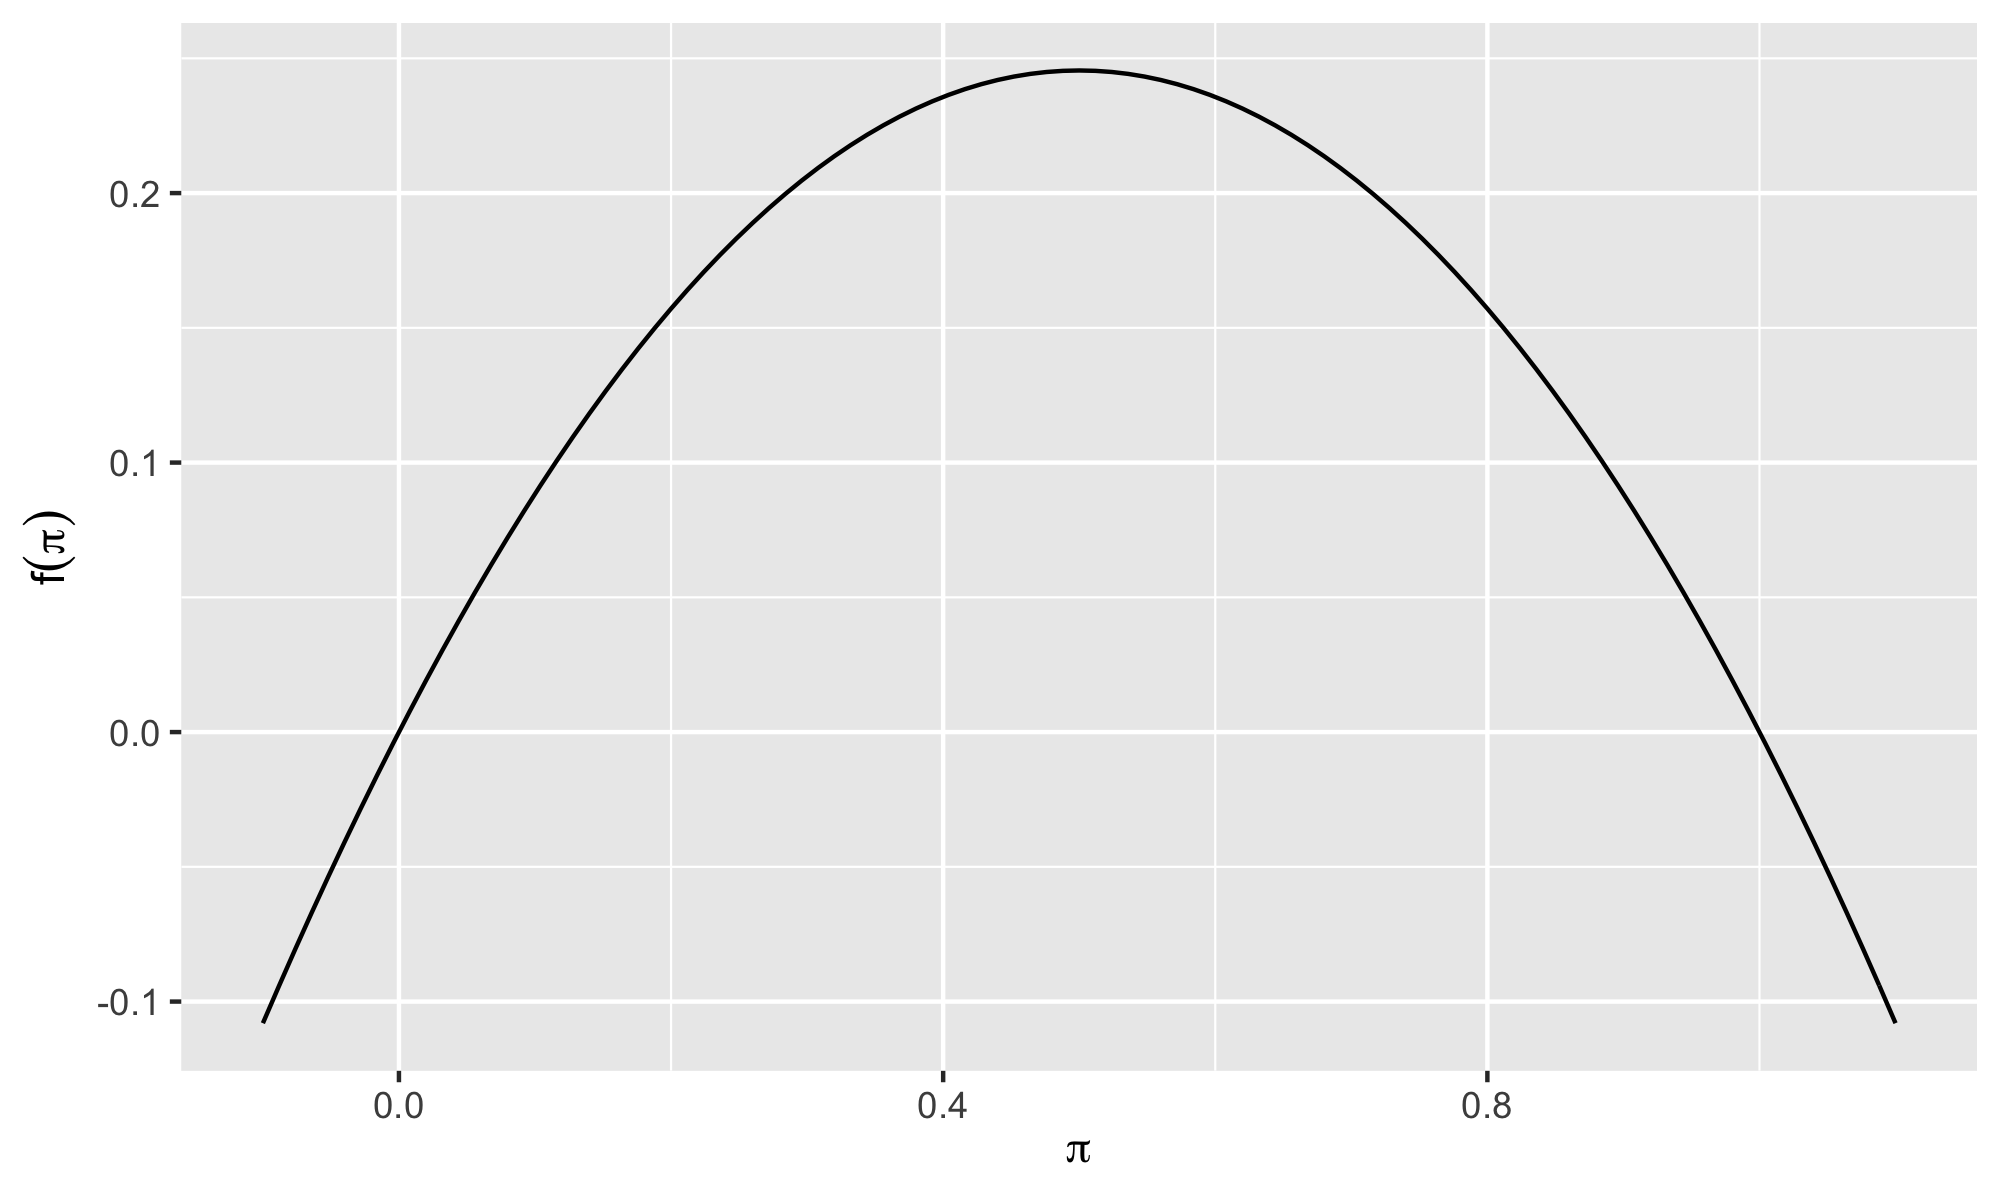
\includegraphics[width=12cm]{f-gate.png}

Similarly, \(LR(E)>1\) for any \(0< \pi <1\). Here is a plot of
\(LR(E)\) against \(\pi\):

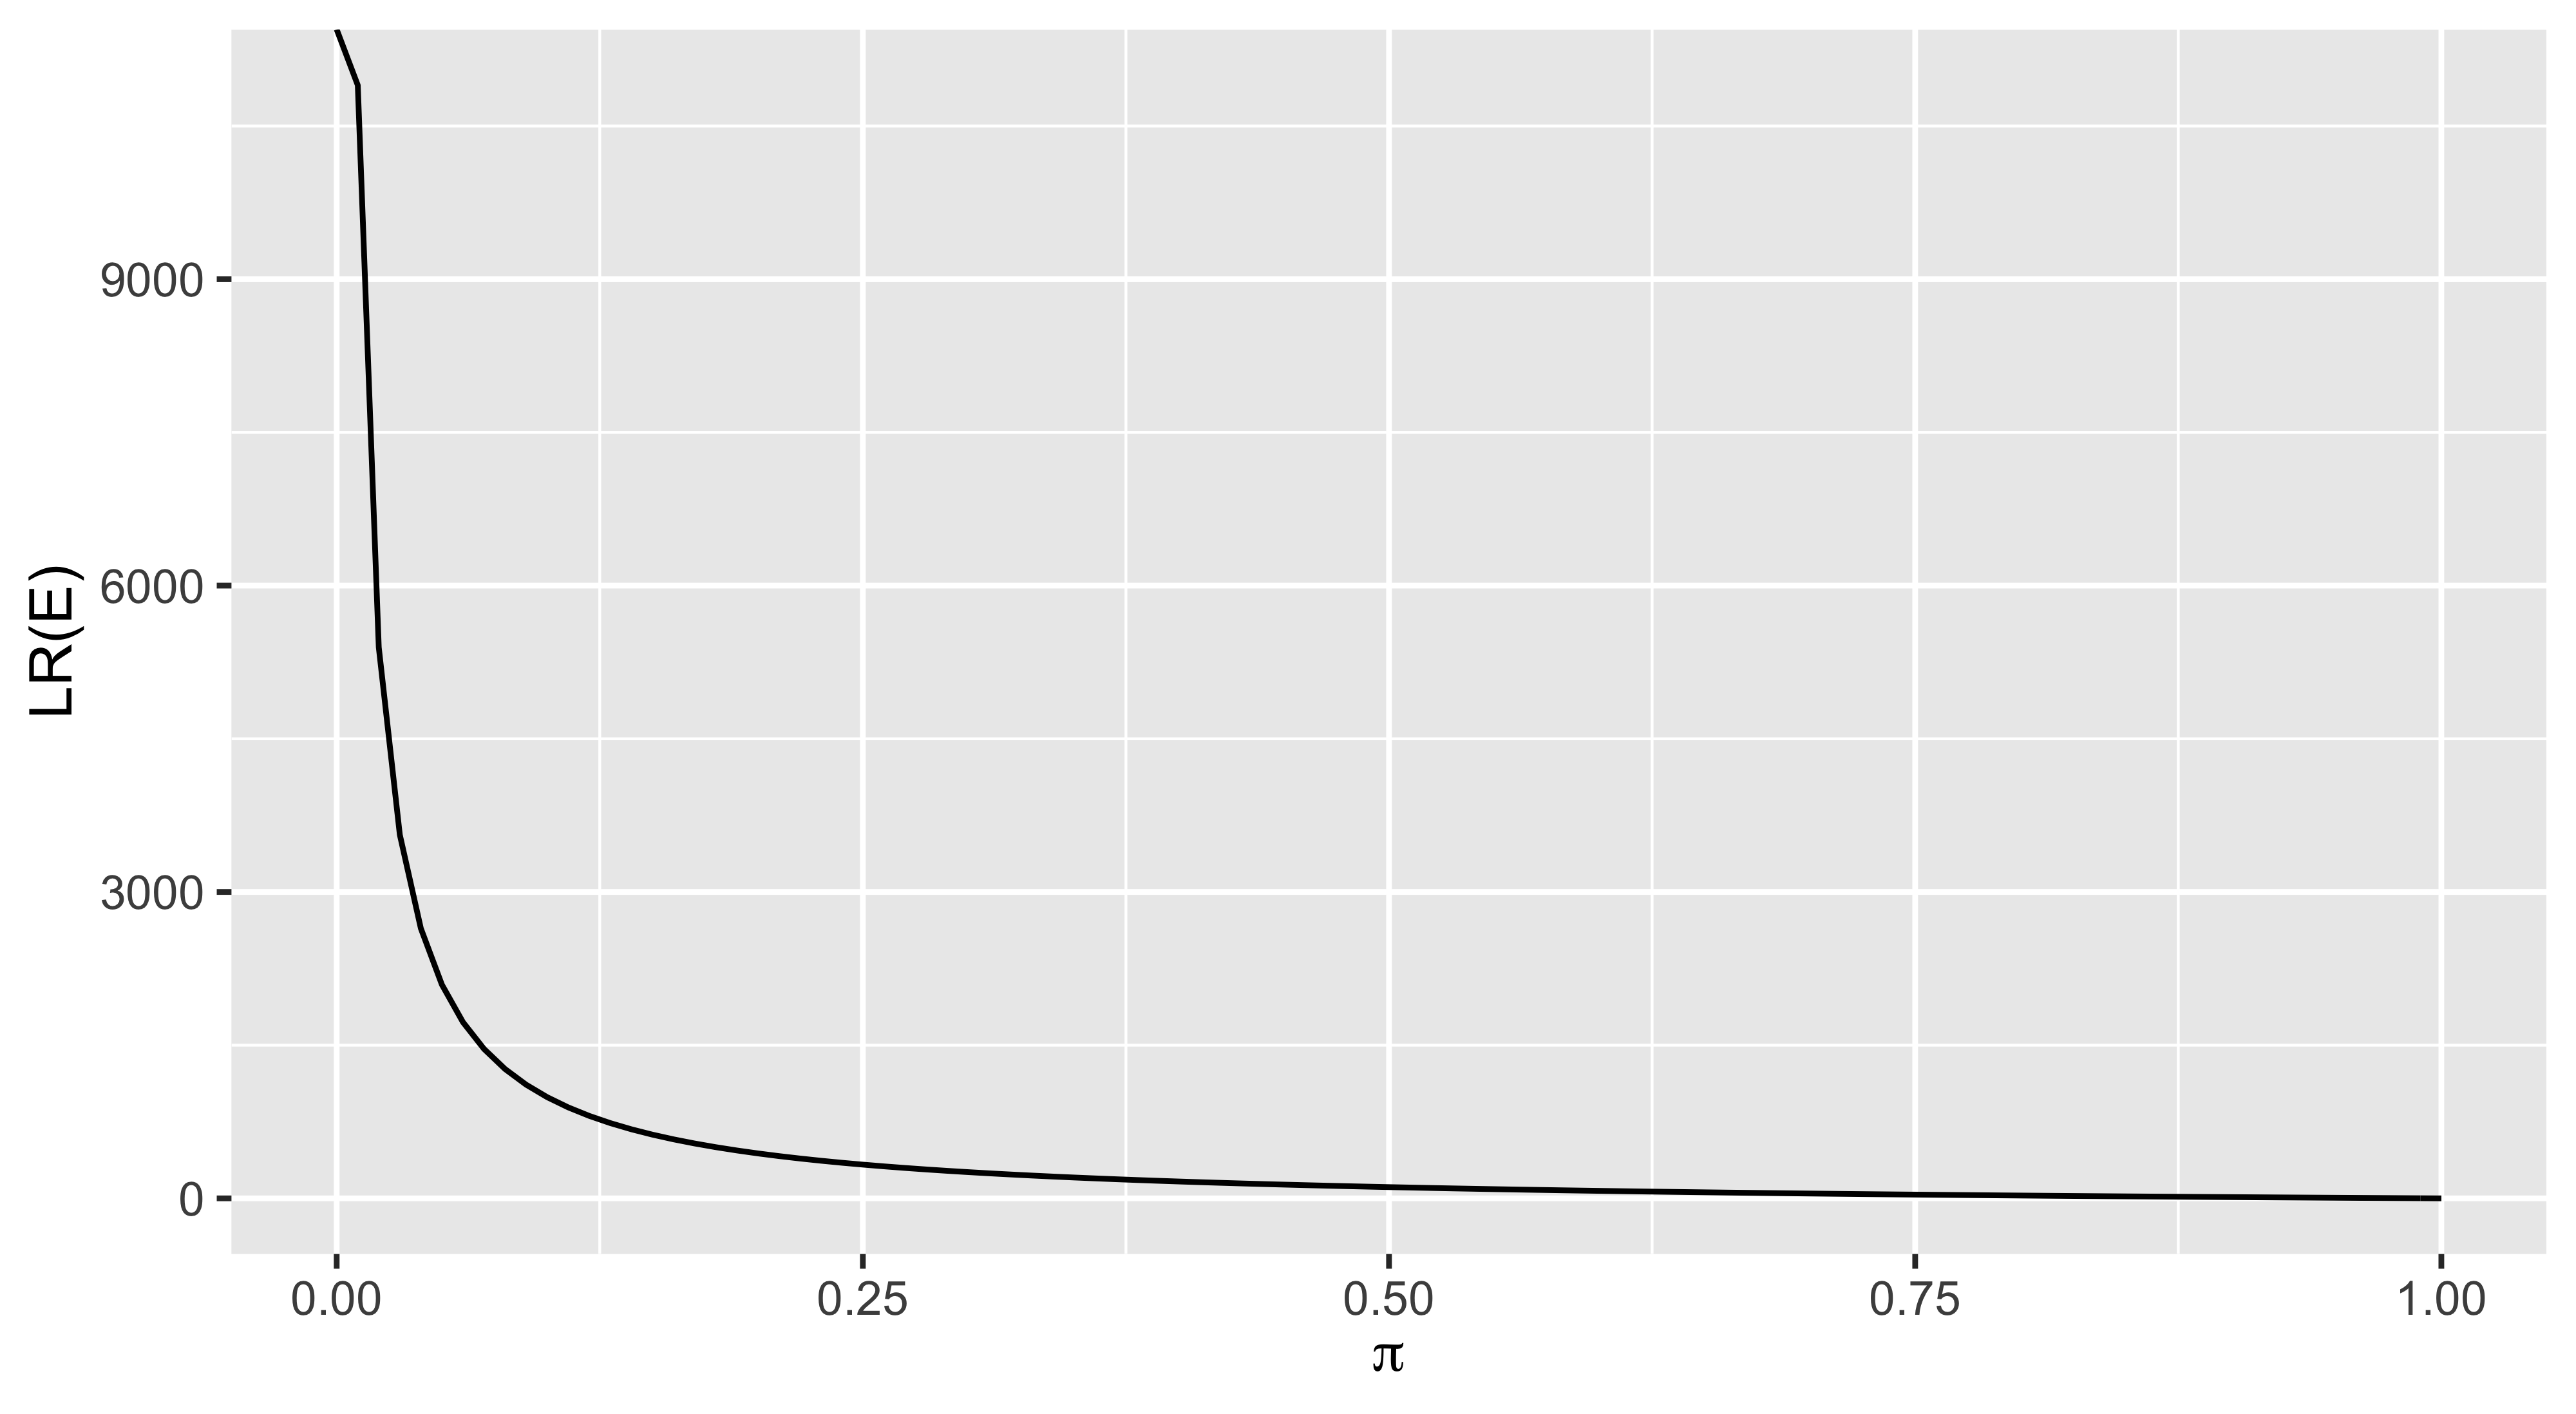
\includegraphics[width=12cm]{lre-gate.png}

\noindent Notice that \(LR(E)\) does not go below 1. This means that for
\(L=G\) in the gatecrasher scenario DTLP wold tell us to convict for any
prior probability of guilt \(\pi\neq 0,1\).

One might ask: is the conclusion very sensitive to the choice of \(L\)
and \(G\)? The answer is, not too much.

\intermezzoa

How sensitive is our analysis to the choice of \(L/G\)? Well, \(LR(E)\)
does not change at all, only the threshold moves. For instance, if
\(L/G=4\), instead of \(f\) we end up with \begin{align*}
 f'(\pi) = - 0.955 \pi^2 + 0.955\pi &>0 
 \end{align*} and the function still takes positive values on the
interval \((0,1)\). In fact, the decision won't change until \(L/G\)
increases to \(\approx 111\). Denote \(L/G\) as \(\rho\), and let us
start with the general decision standard, plugging in our calculations
for \(LR(E)\): \begin{align*}
LR(E) &> \frac{\pr{H_\Delta}}{\pr{H_\Pi}} \rho\\
LR(E) &> \frac{1-\pi}{\pi} \rho \\
\frac{0.991-0.991\pi}{0.009\pi} &> \frac{1-\pi}{\pi} \rho\\
\frac{0.991-0.991\pi}{0.009\pi}\frac{\pi}{1-\pi} &>  \rho\\
\frac{0.991\pi-0.991\pi^2}{0.009\pi-0.009\pi^2} &>  \rho\\
\frac{\pi(0.991-0.991\pi)}{\pi(0.009-0.009\pi)} &>  \rho\\
\frac{0.991-0.991\pi}{0.009-0.009\pi} &>  \rho\\
\frac{0.991(1-\pi)}{0.009(1-\pi)} &>  \rho\\
\frac{0.991}{0.009} &>  \rho\\
110.1111 &>  \rho\\
\end{align*}

\intermezzob

So, we conclude, in usual circumstances, DTLP does not handle the
gatecrasher paradox.

\hypertarget{probabilistic-thresholds-revised}{%
\section{Probabilistic Thresholds
Revised}\label{probabilistic-thresholds-revised}}

\hypertarget{likelihood-ratios-and-naked-statistical-evidence}{%
\subsection{Likelihood ratios and naked statistical
evidence}\label{likelihood-ratios-and-naked-statistical-evidence}}

\hypertarget{conjunction-paradox-and-bayesian-networks}{%
\subsection{Conjunction paradox and Bayesian
networks}\label{conjunction-paradox-and-bayesian-networks}}

\hypertarget{conclusions}{%
\section{Conclusions}\label{conclusions}}

Where are we, how did we get here, and where can we go from here? We
were looking for a probabilistically explicated condition \(\Psi\) such
that the trier of fact, at least ideally, should accept any relevant
claim (including \(G\)) just in case \(\Psi(A,E)\).

From the discussion that transpired it should be clear that we were
looking for a \(\Psi\) satisfying the following desiderata:

\begin{description}
\item[conjunction closure] If $\Psi(A,E)$ and $\Psi(B,E)$, then $\Psi(A\et B,E)$.
\item[naked statistics] The account should at least make it possible for convictions based on strong, but naked statistical evidence to be unjustified. 
\item[equal treatment] the condition should apply to any relevant claim whatsoever (and not just a selected claim, such as $G$).
\end{description}

Throughout the paper we focused on the first two conditions (formulated
in terms of the difficulty about conjunction (DAC), and the gatecrasher
paradox), going over various proposals of what \(\Psi\) should be like
and evaluating how they fare. The results can be summed up in the
following table:

\begin{center}
\footnotesize 
 \begin{tabular}{@{}p{3cm}p{2.5cm}p{4cm}p{3cm}@{}}
\toprule
\textbf{View} & \textbf{Convict iff} & \textbf{DAC} & \textbf{Gatecrasher} \\ \midrule
Threshold-based LP (TLP) & Probability of guilt given the evidence is above a certain threshold & fails & fails \\
Dawid's likelihood strategy & No condition given, focus on $\frac{\pr{H\vert E}}{\pr{H\vert \n E}}$ & - If evidence is fairly reliable, the posterior of $A\et B$ will be greater than the prior.

- The posterior of $A\et B$ can still be lower than the posterior of any of $A$ and $B$.

- Joint likelihood, contrary do Dawid's claim, can also be lower than any of the individual likelihoods. & fails  \\
Cheng's relative LP (RLP)
& Posterior of guilt higher than the posterior of any of the defending narrations & The solution assumes equal costs of errors and independence of $A$ and $B$ conditional on $E$. It also relies on there being multiple defending scenarios individualized in terms of  combinations of literals involving $A$ and $B$. & Assumes that the prior odds of guilt are 1, and that the statistics is not sensitive to guilt (which is dubious). If the latter fails, tells to convict as long as the prior of guilt $<0.991$. \\
Kaplow's decision-theoretic LP (DTLP) &
The likelihood of the evidence is higher than the odds of innocence multiplied by the cost of error ratio & fails & convict if cost ratio $<110.1111$
\end{tabular} 
 \end{center}

Thus, each account either simply fails to satisfy the desiderata, or
succeeds on rather unrealistic assumptions. Does this mean that a
probabilistic approach to legal evidence evaluation should be abandoned?
No.~This only means that if we are to develop a general probabilistic
model of legal decision standards, we have to do better. One promising
direction is to go back to Cohen's pressure against
\textbf{Requirement 1} and push against it. A brief paper suggesting
this direction is (Di Bello, 2019b), where the idea is that the
probabilistic standard (be it a threshold or a comparative wrt.
defending narrations) should be applied to the whole claim put forward
by the plaintiff, and not to its elements. In such a context, DAC does
not arise, but \textbf{equal treatment} is violated. Perhaps, there are
independent reasons to abandon it, but the issue deserves further
discussion. Another strategy might be to go in the direction of
employing probabilistic methods to explicate the narration theory of
legal decision standards (Urbaniak, 2018), but a discussion of how this
approach relates to DAC and the gatecrasher paradox lies beyond the
scope of this paper.

\hypertarget{references}{%
\section{References}\label{references}}

\hypertarget{refs}{}
\leavevmode\hypertarget{ref-Allen1986A-Reconceptuali}{}%
Allen, R. J. (1986). A reconceptualization of civil trials. \emph{Boston
University Law Review}, \emph{66}, 401--437.

\leavevmode\hypertarget{ref-allen2001naturalized}{}%
Allen, R. J., \& Leiter, B. (2001). Naturalized epistemology and the law
of evidence. \emph{Virginia Law Review}, \emph{87}(8), 1491--1550.
JSTOR.

\leavevmode\hypertarget{ref-allen2013}{}%
Allen, R. J., \& Stein, A. (2013). Evidence, probability and the burden
of proof. \emph{Arizona Law Journal}, \emph{55}, 557--602.

\leavevmode\hypertarget{ref-AllenPardo2019relative}{}%
Allen, R., \& Pardo, M. (2019). Relative plausibility and its critics.
\emph{The International Journal of Evidence \& Proof}, \emph{23}(1-2),
5--59. SAGE Publications. Retrieved from
\url{https://doi.org/10.1177/1365712718813781}

\leavevmode\hypertarget{ref-arkesEtAl2012}{}%
Arkes, H. R., Shoots-Reinhard, B. L., \& Mayes, R. S. (2012).
Disjunction between probability and verdict in juror decision making.
\emph{Journal of Behavioral Decision Making}, \emph{25}(3), 276--294.

\leavevmode\hypertarget{ref-Bernoulli1713Ars-conjectandi}{}%
Bernoulli, J. (1713). \emph{Ars conjectandi}.

\leavevmode\hypertarget{ref-BlomeTillmann2017}{}%
Blome-Tillmann, M. (2017). ``More likely than not'' --- Knowledge first
and the role of bare statistical evidence in courts of law. In A.
Carter, E. Gordon, \& B. Jarvi (Eds.), \emph{Knowledge
first---approaches in epistemology and mind} (pp. 278--292). Oxford
University Press. Retrieved from
\url{https://doi.org/10.1093/oso/9780198716310.003.0014}

\leavevmode\hypertarget{ref-bolinger2018rational}{}%
Bolinger, R. (2018). The rational impermissibility of accepting (some)
racial generalizations. \emph{Synthese}, 1--17. Springer.

\leavevmode\hypertarget{ref-buchak2014belief}{}%
Buchak, L. (2014). Belief, credence, and norms. \emph{Philosophical
Studies}, \emph{169}(2), 285--311.

\leavevmode\hypertarget{ref-cheng2012reconceptualizing}{}%
Cheng, E. (2012). Reconceptualizing the burden of proof. \emph{Yale LJ},
\emph{122}, 1254. HeinOnline.

\leavevmode\hypertarget{ref-Cohen1977The-probable-an}{}%
Cohen, J. (1977). \emph{The probable and the provable}. Oxford
University Press.

\leavevmode\hypertarget{ref-cohen1988difficulty}{}%
Cohen, L. J. (1988). The difficulty about conjunction in forensic proof.
\emph{The Statistician}, \emph{37}(4/5), 415. JSTOR. Retrieved from
\url{https://doi.org/10.2307/2348767}

\leavevmode\hypertarget{ref-dawid1987difficulty}{}%
Dawid, A. P. (1987). The difficulty about conjunction. \emph{The
Statistician}, 91--97. JSTOR.

\leavevmode\hypertarget{ref-Dekay1996}{}%
Dekay, M. L. (1996). The difference between Blackstone-like error ratios
and probabilistic standards of proof. \emph{Law and Social Inquiry},
\emph{21}, 95--132.

\leavevmode\hypertarget{ref-dhamiEtAl2015}{}%
Dhami, M. K., Lundrigan, S., \& Mueller-Johnson, K. (2015). Instructions
on reasonable doubt: Defining the standard of proof and the jurors task.
\emph{Psychology, Public Policy, and Law, 21(2), 169178}, \emph{21}(2),
169--178.

\leavevmode\hypertarget{ref-diamond90}{}%
Diamond, H. A. (1990). Reasonable doubt: To define, or not to define.
\emph{Columbia Law Review}, \emph{90}(6), 1716--1736.

\leavevmode\hypertarget{ref-diBello2019}{}%
Di Bello, M. (2019a). Trial by statistics: Is a high probability of
guilt enough to convict? \emph{Mind}.

\leavevmode\hypertarget{ref-DiBello2019plausibility}{}%
Di Bello, M. (2019b). Probability and plausibility in juridical proof.
\emph{International Journal of Evidence and Proof}.

\leavevmode\hypertarget{ref-ebert2018}{}%
Ebert, P. A., Smith, M., \& Durbach, I. (2018). Lottery judgments: A
philosophical and experimental study. \emph{Philosophical Psychology},
\emph{31}(1), 110--138.

\leavevmode\hypertarget{ref-Enoch2012Statistical}{}%
Enoch, D., Spectre, L., \& Fisher, T. (2012). Statistical evidence,
sensitivity, and the legal value of knowledge. \emph{Philosophy and
Public Affairs}, \emph{40}(3), 197--224.

\leavevmode\hypertarget{ref-friedman2015}{}%
Friedman, O., \& Turri, J. (2015). Is probabilistic evidence a source of
knowledge? \emph{Cognitive Science}, \emph{39}(5), 1062--1080.

\leavevmode\hypertarget{ref-haack2011legal}{}%
Haack, S. (2014). Legal probabilism: An epistemological dissent. In
\emph{Haack2014-HAAEMS} (pp. 47--77).

\leavevmode\hypertarget{ref-HeddenColyvan2019legal}{}%
Hedden, B., \& Colyvan, M. (2019). Legal probabilism: A qualified
defence. \emph{Journal of Political Philosophy}, \emph{27}(4), 448--468.
Wiley. Retrieved from \url{https://doi.org/10.1111/jopp.12180}

\leavevmode\hypertarget{ref-ho2008philosophy}{}%
Ho, H. L. (2008). \emph{A philosophy of evidence law: Justice in the
search for truth}. Oxford University Press.

\leavevmode\hypertarget{ref-Horowitz1996}{}%
Horowitz, I. A., \& Kirkpatrick, L. C. (1996). A concept in search of a
definition: The effect of reasonable doubt instrcutions on certainty of
guilt standards and jury verdicts. \emph{Law and Human Behaviour},
\emph{20}(6), 655--670.

\leavevmode\hypertarget{ref-Kaplan1968decision}{}%
Kaplan, J. (1968). Decision theory and the fact-finding process.
\emph{Stanford Law Review}, \emph{20}(6), 1065--1092.

\leavevmode\hypertarget{ref-kaplow2014likelihood}{}%
Kaplow, L. (2014). Likelihood ratio tests and legal decision rules.
\emph{American Law and Economics Review}, \emph{16}(1), 1--39. Oxford
University Press.

\leavevmode\hypertarget{ref-kaye79}{}%
Kaye, D. H. (1979a). The laws of probability and the law of the land.
\emph{The University of Chicago Law Review}, \emph{47}(1), 34--56.

\leavevmode\hypertarget{ref-Kaye79gate}{}%
Kaye, D. H. (1979b). The paradox of the Gatecrasher and other stories.
\emph{The Arizona State Law Journal}, 101--110.

\leavevmode\hypertarget{ref-Laplace1814}{}%
Laplace, P. (1814). \emph{Essai philosophique sur les probabilités}.

\leavevmode\hypertarget{ref-laudan2006truth}{}%
Laudan, L. (2006). \emph{Truth, error, and criminal law: An essay in
legal epistemology}. Cambridge University Press.

\leavevmode\hypertarget{ref-laudan2016law}{}%
Laudan, L. (2016). \emph{The law's flaws: Rethinking trials and errors?}
Law and society. College Publications. Retrieved from
\url{https://books.google.pl/books?id=MvkWvgAACAAJ}

\leavevmode\hypertarget{ref-Lempert1986}{}%
Lempert, R. O. (1986). The new evidence scholarship: Analysing the
process of proof. \emph{Boston University Law Review}, \emph{66},
439--477.

\leavevmode\hypertarget{ref-Loftus1996}{}%
Loftus, E. F. (1996). \emph{Eyewitness testimony (revised edition)}.
Harvard University Press.

\leavevmode\hypertarget{ref-moss2018}{}%
Moss, S. (2018). \emph{Probabilistic knowledge}. Oxford University
Press.

\leavevmode\hypertarget{ref-Nesson1979Reasonable-doub}{}%
Nesson, C. R. (1979). Reasonable doubt and permissive inferences: The
value of complexity. \emph{Harvard Law Review}, \emph{92}(6),
1187--1225.

\leavevmode\hypertarget{ref-newman1993}{}%
Newman, J. O. (1993). Beyon ``reasonable doub''. \emph{New York
University Law Review}, \emph{68}(5), 979--1002.

\leavevmode\hypertarget{ref-niedermeierEtAl1999}{}%
Niedermeier, K. E., Kerr, N. L., \& Messeé, L. A. (1999). Jurors' use of
naked statistical evidence: Exploring bases and implications of the
Wells effect. \emph{Journal of Personality and Social Psychology},
\emph{76}(4), 533--542.

\leavevmode\hypertarget{ref-nunn2015}{}%
Nunn, A. G. (2015). The incompatibility of due process and naked
statistical evidence. \emph{Vanderbilt Law Review}, \emph{68}(5),
1407--1433.

\leavevmode\hypertarget{ref-pardo2018}{}%
Pardo, M. S. (2018). Safety vs.~Sensitivity: Possible worlds and the law
of evidence. \emph{Legal Theory}, \emph{24}(1), 50--75.

\leavevmode\hypertarget{ref-pritchard2005epistemic}{}%
Pritchard, D. (2005). \emph{Epistemic luck}. Clarendon Press.

\leavevmode\hypertarget{ref-pundik2017}{}%
Pundik, A. (2017). Freedom and generalisation. \emph{Oxford Journal of
Legal Studies}, \emph{37}(1), 189--216.

\leavevmode\hypertarget{ref-redmayne2008exploring}{}%
Redmayne, M. (2008). Exploring the proof paradoxes. \emph{Legal Theory},
\emph{14}(4), 281--309. Cambridge University Press.

\leavevmode\hypertarget{ref-Roth2010}{}%
Roth, A. (2010). Safety in numbers? Deciding when DNA alone is enough to
convict. \emph{New York University Law Review}, \emph{85}(4),
1130--1185.

\leavevmode\hypertarget{ref-schwartz2017ConjunctionProblemLogic}{}%
Schwartz, D. S., \& Sober, E. R. (2017). The Conjunction Problem and the
Logic of Jury Findings. \emph{William \& Mary Law Review}, \emph{59}(2),
619--692.

\leavevmode\hypertarget{ref-smith2017}{}%
Smith, M. (2018). When does evidence suffice for conviction?
\emph{Mind}, \emph{127}(508), 1193--1218.

\leavevmode\hypertarget{ref-Stein05}{}%
Stein, A. (2005). \emph{Foundations of evidence law}. Oxford University
Press.

\leavevmode\hypertarget{ref-sykes1999}{}%
Sykes, D. L., \& Johnson, J. T. (1999). Probabilistic evidence versus
the representation of an event: The curious case of Mrs. Prob's dog.
\emph{Basic and Applied Social Psychology}, \emph{21}(3), 199--212.

\leavevmode\hypertarget{ref-thomson1986liability}{}%
Thomson, J. J. (1986). Liability and individualized evidence. \emph{Law
and Contemporary Problems}, \emph{49}(3), 199--219. JSTOR.

\leavevmode\hypertarget{ref-urbaniak2018narration}{}%
Urbaniak, R. (2018). Narration in judiciary fact-finding: A
probabilistic explication. \emph{Artificial Intelligence and Law},
1--32.

\leavevmode\hypertarget{ref-walen2015}{}%
Walen, A. (2015). Proof beyond a reasonable doubt: A balanced
retributive account. \emph{Louisiana Law Review}, \emph{76}(2),
355--446.

\leavevmode\hypertarget{ref-wasserman1991morality}{}%
Wasserman, D. T. (1991). The morality of statistical proof and the risk
of mistaken liability. \emph{Cardozo L. Rev.}, \emph{13}, 935.
HeinOnline.

\leavevmode\hypertarget{ref-wells1992naked}{}%
Wells, G. (1992). Naked statistical evidence of liability: Is subjective
probability enough? \emph{Journal of Personality and Social Psychology},
\emph{62}(5), 739--752. American Psychological Association.

\end{document}
